\documentclass[journal]{IEEEtran}

\usepackage{cite}
\usepackage{graphicx}
\graphicspath{{./} {fig/}}
% \usepackage[tight,footnotesize]{subfigure}
\usepackage{caption}
\captionsetup[figure]{font=small}
\captionsetup[table]{textfont={sc,footnotesize}, labelfont=footnotesize, labelsep=newline, justification=centering} %ieee table format
\usepackage{subcaption}
\renewcommand\thesubfigure{(\alph{subfigure})} %引用子图格式：数字(字母)，如Fig.1(a)
\DeclareCaptionLabelFormat{opening}{#2}
\captionsetup[subfigure]{labelformat=opening} %避免子图出现双括号

\usepackage{amsmath}
\usepackage{algorithmic}
\usepackage{url}
\usepackage{array}

\usepackage{threeparttable}
\usepackage{tabularx}
\usepackage{booktabs}
\usepackage[table,xcdraw]{xcolor}
\usepackage{adjustbox}
\usepackage[utf8]{inputenc}

\usepackage{acronym}
\usepackage{multirow}
\usepackage{algorithm}
\usepackage{algorithmic}
\newcommand{\chicca}[1]{{\color{red}{\bf elisabetta:} #1}}

%% Block comment. \begin{comment}  \end{comment}
\usepackage{verbatim}

%% Provides generic commands \degree, \celsius, \perthousand, \micro and \ohm which work both in text and maths mode.
\usepackage{textcomp,gensymb}

%% line break
\usepackage{makecell}

%% 调整表格线与上下内容的间隔
\usepackage{booktabs}

%% emphasizing text 
\usepackage{soul}
\setstcolor{red}
\hyphenation{op-tical net-works semi-conduc-tor}

\begin{document}

% paper title
% Linebackers \\ can be used within to get better formatting as desired.
% Do not put math or special symbols in the title.
\title{A Robust Time-based Multi-level Sensing Circuit for Resistive Memory}


% author names and affiliations
% use a multiple column layout for up to three different
% affiliations
\author{
        Xueyong~Zhang, Byungkwon An,
        % Xueyong~Zhang,~\IEEEmembership{Student~Member,~IEEE,}
        and~Tony~Tae-Hyoung~Kim,~\IEEEmembership{Senior Member,~IEEE}% <-this % stops a space
\thanks{
Manuscript received August 11, 2021; revised August 11, 2021. Date of publication August 11, 2021; date of current version August 11, 2021. This paper was recommended by Associate Editor XXX. 
}% <-this % stops a space}
\thanks{
% Q. Wang and J.Wang are with the College of Telecommunications and Information Engineering, Nanjing University of Posts and Telecommunications, China. \par
% X. Zhang and A. Basu 
The authors are with the School of Electrical and Electronic Engineering, Nanyang Technological University, Singapore 639798 (e-mail: xueyong001@e.ntu.edu.sg; E190209@e.ntu.edu.sg; thkim@ntu.edu.sg).
}% <-this % stops a space}
\thanks{
Color versions of one or more of the figures in this article are available online at http://ieeexplore.ieee.org. \par
Digital Object Identifier xxx
}
}

\maketitle
\IEEEpeerreviewmaketitle

\begin{abstract}
Resistive random access memory (RRAM) is a promising emerging nonvolatile memory (NVM) due to its large resistance ratio in different switching states. To improve memory density and reduce cost-per-bit, multi-level cell (MLC) RRAM stores multiple bits in a single cell, compared to a single-level cell (SLC). However, random mismatch, process variation, and resistance shift lead to reliability issues, degrade the probability of correct read, and increase the bit error rate (BER). 
This paper presents a time-based sensing scheme for robust read operation and extends to multi-level sensing for SLC and MLC RRAM arrays. Bit line (BL) voltage is converted into time delay by a voltage-to-time converter (VTC) and compared with the implicit timing reference generated by a delay line. By detecting different states in the time domain, the proposed time-mode sense amplifier (TSA) requires no analog reference voltage or current, which is used in the conventional voltage-mode sense amplifiers (VSA) or current-mode sense amplifiers (CSA). Power gating is employed to enable the time sampling only at the sensing points to suppress the short-circuit current. A charge sharing-induced error compensation (CSEC) circuit is used to eliminate the charge sharing-induced voltage drop and expand the sense margin by 1.56$\times$.
Monte Carlo simulations in 40nm technology show that the proposed TSA improves read reliability and reduces BER by 3-4 orders of magnitude compared to conventional VSA and CSA. 
The proposed time-based sensing scheme operates from 0.7-1.2 V supply and consumes 49 fJ/bit for read operation under a nominal 1.2 V supply.

% \textcolor{red}{1.2 V}

\end{abstract}
 
\begin{IEEEkeywords}
Nonvolatile memory (NVM), 
resistive random access memory (RRAM),
multi-level cell (MLC),
time-based SA,
robust sensing.
\end{IEEEkeywords}

\section{Introduction}
\label{sec_intro}
% \IEEEPARstart{A}{}demo file is ....

\IEEEPARstart{T}{he} improvements in memory density and computing performance resulting from CMOS scaling are shrinking since the transistor size is approaching its physical limitation. To further improve computing capability and reduce power consumption, various emerging non-volatile memory (NVM) devices are promoted, utilizing various physical properties such as ionic migration \cite{waser2010nanoionics}, phase transition \cite{wuttig2007phase}, or spintronics \cite{6853380}. They store information in the format of two or more distinct resistance states.
Resistive random access memory (RRAM) has a metal-insulator-metal (MIM) sandwich structure, where data are represented by the resistance of a conductive filament (CF) formed in the insulator (metal-oxide layer) \cite{7448912}. The formation of a CF leads to the low resistance state (LRS) by SET operation while the rupture of CF switches to the high resistance state (HRS) by RESET operation.  
With the features of relatively high density ($\sim$ 4 F$^2$/bit), high speed ($\sim$ 5 ns), ultra-low energy ($\leq$ pJ), and large resistance ratio ($10 \sim 1000$) \cite{6361301, 2019Emerging}, RRAM is considered as an excellent NVM device to implement multiplication-and-accumulation (MAC) computation in in-memory computing (IMC) architectures \cite{7950949, 8998360, 9335229} and artificial synapse in neuromorphic hardware systems \cite{8705375, 7423754, 8340055, 9369873}.

In actual experiments, however, the resistances in HRS/LRS and the voltages for set/reset operation between cycle to cycle (C2C) and device to device (D2D) vary because of the broad fluctuations of CF in RRAM device, which introduce variation and uncertainty. 
As a result, special circuitry is required for robust write and read operation. This work focuses on robust sensing circuit design for read operation to improve read reliability and reduce read bit error rate (BER).

% %% figure of section II
% \begin{figure*}[!t]
% \centerline
% {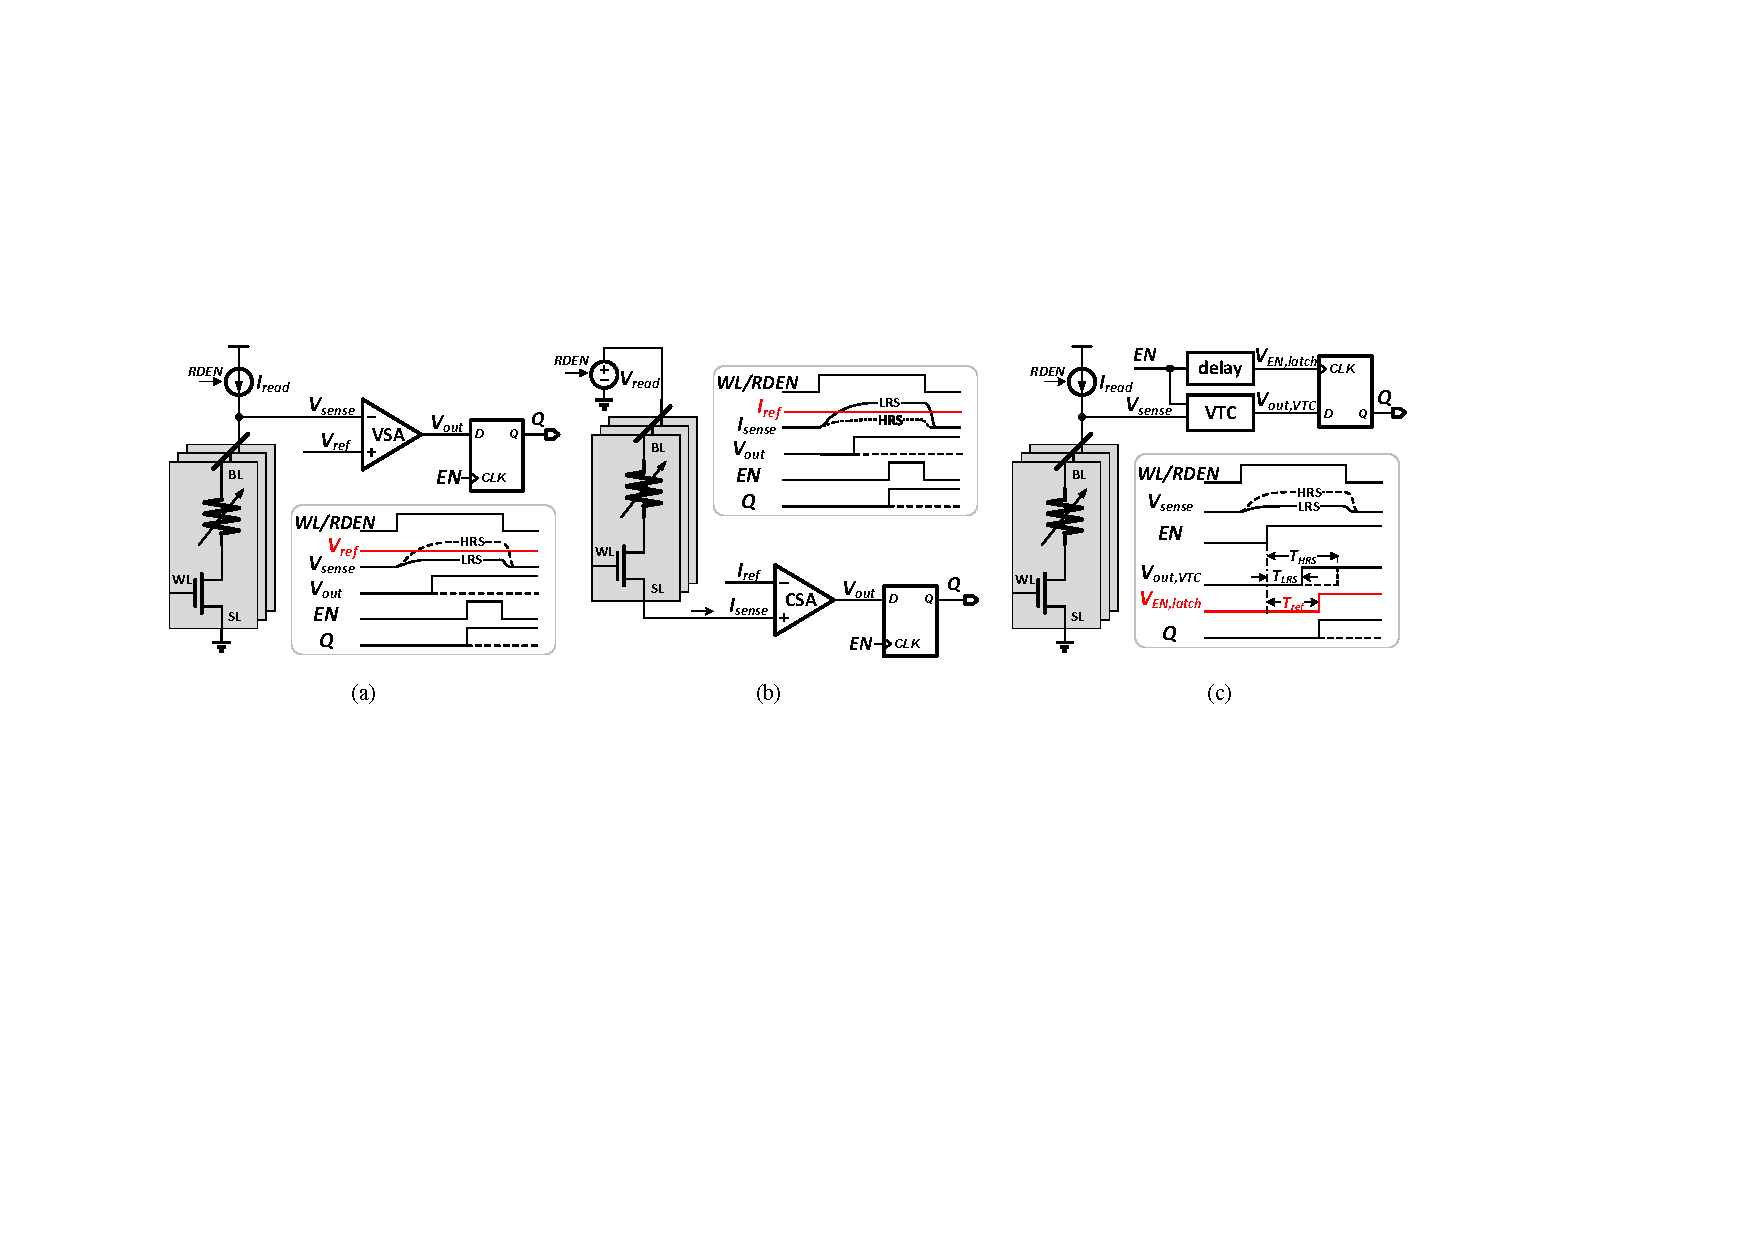
\includegraphics[width=0.95\textwidth]{fig/SA_types.pdf}}
% \caption{Conceptual circuit schematics of three different sensing schemes for NVM array. (a) Voltage mode, (b) Current mode, (c) Time mode. Assuming one specific column-wise bit line (BL) is selected.}
% \label{fig_sensing_mode}
% \end{figure*}

As a type of NVM, RRAM is suitable for applications with infrequent write operations and frequent read operations.
The energy consumption of an RRAM-based system depends largely on the readout sensing mechanism \cite{wan2020voltage}.
Therefore, the sensing performance is one of the most critical evaluations.
In general, there are three different ways to sense the data stored in RRAM by converting the data into voltage, current, and time respectively \cite{8906921}. 
% \textcolor{blue}{
The commonly used voltage mode sense amplifier (VSA) is an inverter-based latch structure \cite{yang20132mb}. However, the speed of VSA is slow, especially when bitline (BL) is too long and the resistance of RRAM in LRS is too high.
To increase the sense margin, \cite{chang201419} proposed a swing-sample-and-couple (SSC) VSA. However, the offset current affects the sensing performance. An offset-canceling (OC) current mode sense amplifier (CSA) was proposed in \cite{jain201913}. The effect of offset on the data path is eliminated by cross-sampling.
To achieve a short access time and tolerate a small read margin, \cite{lo2018reram} proposes a dynamic-trip-point-mismatch-sampling (DTPMS) CSA with small offset current and early sensing. 
On the other hand, \cite{8906921} presented a time-based sensing scheme by converting the current drawn from the bitcell to voltage pulses, which can easily distinguish the states of multi-level cell (MLC). However, the read time is too long since the number of pulses is proportional to the current’s magnitude.
% }

In this paper, we propose a novel time-based low power sensing scheme for robust reading, where the bit line (BL) voltage is converted into time delay.
It can be used for all two-terminal NVM technologies (e.g., STT-RAM, PCM, and RRAM), whose states are differentiated by the switching between a high resistance state (off-state) and a low resistance state (on-state). 
The proposed time-based sensing scheme improves the read robustness and accuracy by converting the bitcell state into time domain with the features of low power consumption and low read BER. The controller supports two different sensing modes for automatic readout. The design is scalable to multi-level sensing (MLS) that can distinguish the states of MLC. The main contributions are summarized as follows.
\begin{itemize}
  \item [1)] 
  In section \ref{sec_conv}, we describe the adopted simulation framework and clarify the particularity of the RRAM sensing methodology. The common sensing schemes based on the voltage, current, and time-domain are reviewed and compared.  
  \item [2)]
  In section \ref{sec_prop}, a time-based sensing scheme is proposed to improve the read reliability and reduce read BER. The circuit implementation and design trade-offs are analyzed. Charge-sharing-induced error compensation (CSEC) circuit is introduced to suppress charge sharing-induced error and enlarge the voltage margin of HRS and LRS, making RRAM state sensing easier and more accurate. The power gating technique enables the shaping inverter only at the sensing point to limit the short-circuit current, which is the main source of power consumption. Two operation modes of RRAM reading are supported by the timing controller circuit.
  \item [3)]
  In section \ref{sec_features}, we extend the proposed sensing scheme to MLS. This can improve sensing accuracy further by separating the sensing points for HRS and LRS. The MLS can discriminate multiple states to support MLC sensing. 
  \item [4)]
  In section \ref{sec_results}, we explore the circuit design knobs to optimize the overall performance. The simulation results are evaluated and compared with prior works. 
 %related simulation results are discussed.
  \item [5)]
  In section \ref{sec_conclusion}, we conclude this paper and summarize the benefits of the time-based sensing technique.
\end{itemize}

% The remainder of the paper is structured as follows. First, RRAM array design and the common sensing schemes are . Section \ref{sec:prop} discusses the proposed switch capacitor based PI structure and analyses the working principle. The multi-bit scaling is also discussed. Section \ref{sec:results} presents measurement results of the prototype and shows a performance comparison. Finally, the conclusions are provided in section \ref{sec:conclusion}.

\section{RRAM Model and Conventional Sensing Schemes}
\label{sec_conv}
Because of the features of nonvolatile, very high density, and ultra-low power consumption, the emerging RRAM is believed to be a promising candidate for nonvolatile storage, in-memory computing, and neuromorphic applications. However, unstable device performance poses a challenge in reliable sensing and requires a special circuit structure for improving the sensing capability. 
An accurate RRAM circuit model including variations is also critical in designing a reliable sensing circuit. 

% The configuration of a one-transistor-one-RRAM (1T1R) cell is widely used in memory array design, in which one dedicated transistor controls the access of the RRAM device and complies the device current.

\subsection{RRAM Model and Simulation Framework}
\label{sim_model}
% An accuracy RRAM circuit model is the foundation of the study. 
In this work, we employ a simulation framework and the device models that are similar to \cite{9234102} and \cite{lu2020reram}. 
Table \ref{tab_model} summarizes key fundamental RRAM parameters that are used in our analysis. 
A commercial 40-nm standard CMOS design kit is utilized for transistors.
Post layout simulation and analysis are performed to optimize the design.


\begin{figure}[!t]
\centerline
{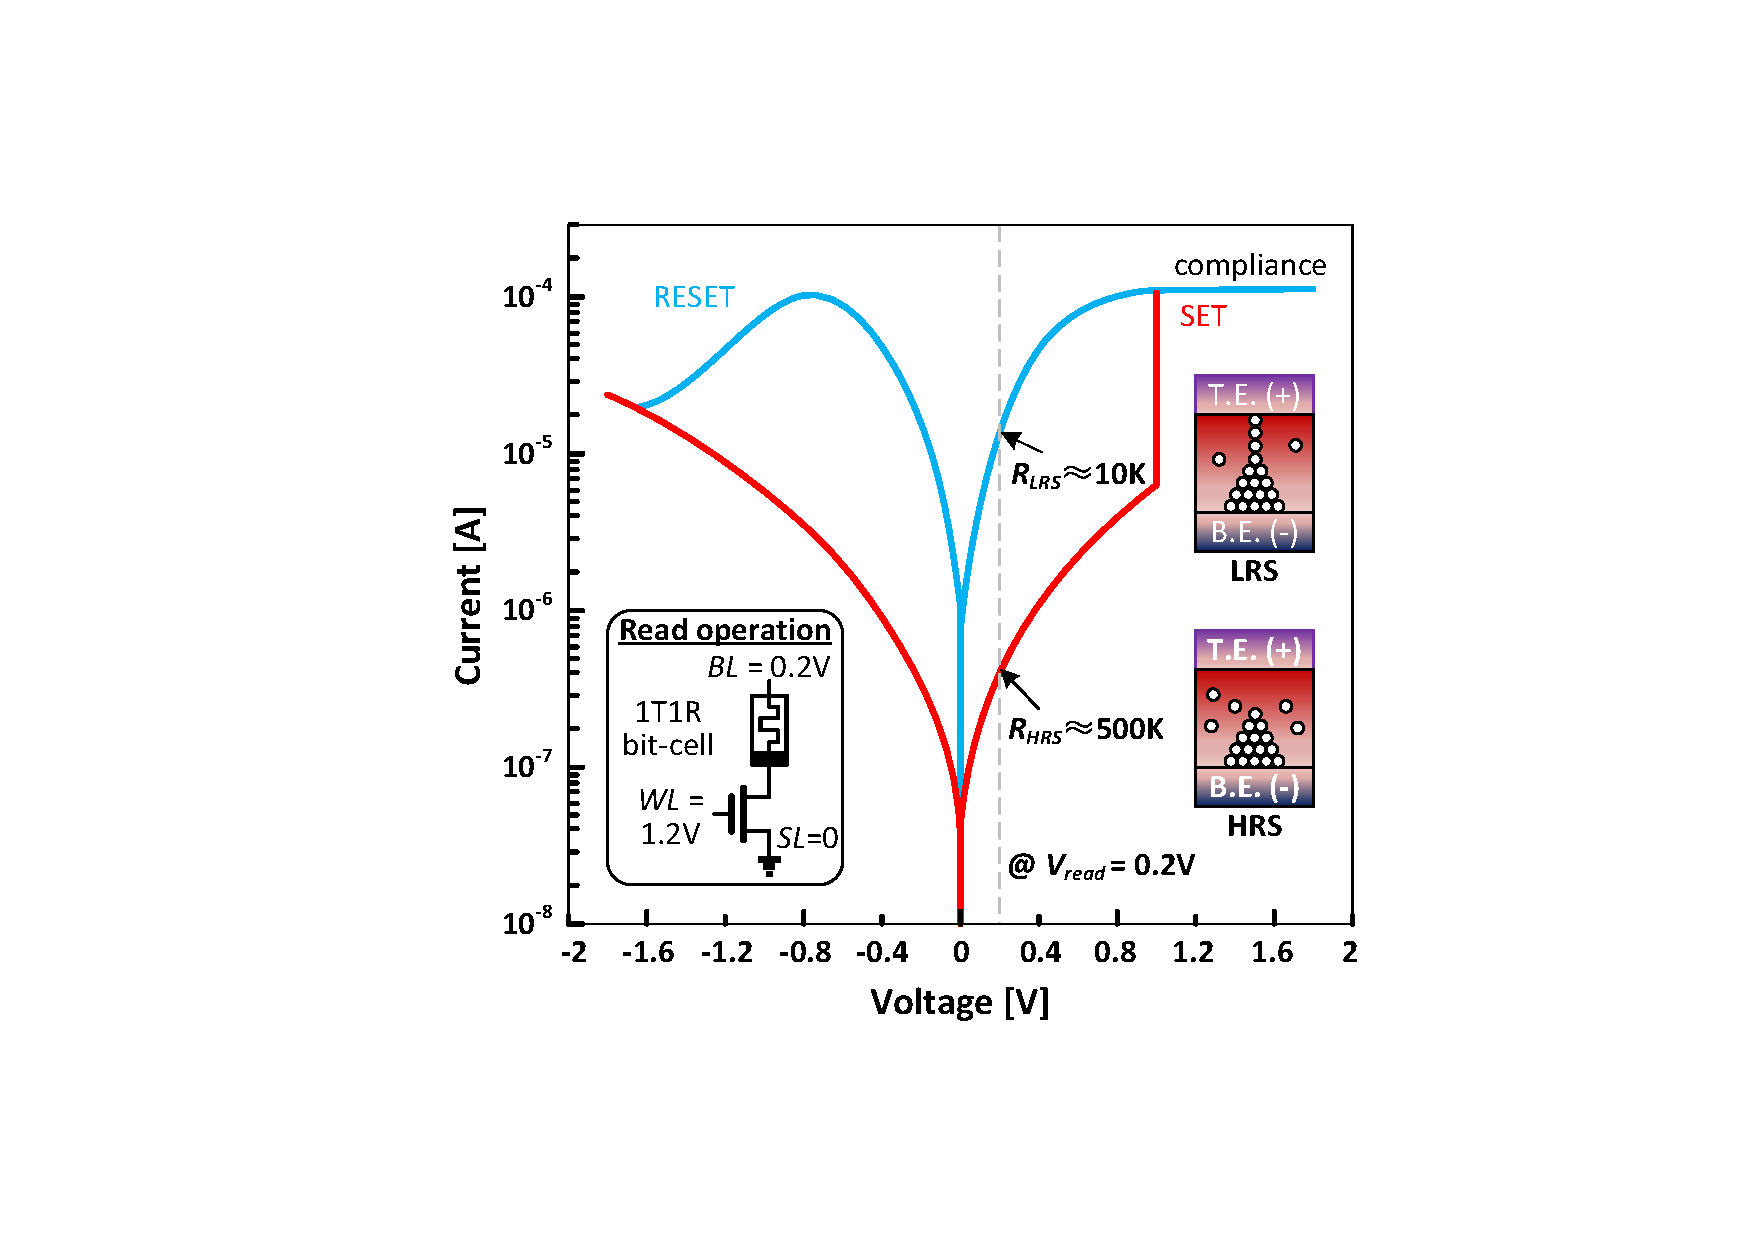
\includegraphics[width=0.45\textwidth]{RRAM_IV_curve.pdf}}
\caption{The model simulation results of the RRAM DC I-V characteristic curves and read operation settings. The resistances of HRS and LRS are 500 K$\Omega$ and 10 K$\Omega$ respectively under the read voltage of 0.2 V.}
\label{IV_curve}
\end{figure}


\begin{table}[!t]
\centering
\caption{Key Parameters for Employed RRAM Device}
\label{tab_model}
 \begin{threeparttable}
% \begin{tabular}{|c{1.3cm}|p{1.5cm}|p{1.6cm}|p{1.3cm}|p{2cm}|p{1.3cm}|p{1.3cm}|p{5cm}|}
\begin{tabular}{@{}m{5cm}<{\centering}|m{2.5cm}<{\centering}@{}}
% \begin{tabular}{lllllll}
\toprule[1.5pt]
\hline
% This work & 65 & Differential, 4-stage  & 0.11-0.38\tnote{1}  & 80   \\\hline
RRAM size ($W\times L$)     & 100 nm $\times$ 100 nm  \\\hline
nominal resistance of HRS ($R_{HRS}$)   & 500 K$\Omega$  \\\hline
standard deviation of $R_{HRS}$   & 100 K$\Omega$  \\\hline
nominal resistance of LRS ($R_{LRS}$)  & 10 K$\Omega$  \\\hline
standard deviation of $R_{LRS}$   & 2 K$\Omega$  \\\hline
nominal set voltage ($V_{SET}$)        & 0.8 V  \\\hline
standard deviation of $V_{SET}$        & 0.15 V  \\\hline
nominal reset voltage ($V_{RESET}$)      & -1.1 V  \\\hline
standard deviation of $V_{RESET}$        & 0.225 V  \\\hline
read voltage ($V_{read}$)	& $0.2V$  \\\hline
temperature coefficient of $R_{HRS}$	& -0.0015  \\\hline
temperature coefficient of $R_{LRS}$	& 0.001  \\\hline
\bottomrule[1.5pt]
\end{tabular}
% \begin{tablenotes}
% \item[1] Excluding V-I converter power 
% \end{tablenotes}
\end{threeparttable}
\end{table} 
 

To restrain the sneak current of the half-selected cells, one common way to implement RRAM bit cells in an array is to integrate an RRAM device in series with a MOS transistor. This is known as the 1T1R structure \cite{6936923} where one dedicated transistor controls the access of the RRAM device and complies the device current.
Fig. \ref{IV_curve} shows the typical current-voltage (I-V) characteristic curves of an $HfO_x$ based RRAM with a cell size of $100\times 100$ nm$^2$. The red and blue curves represent HRS and LRS, respectively, whose resistances are 500 K and 10 K when the read voltage is 0.2 V. The left bottom of Fig. \ref{IV_curve} shows the read operation setting of the 1T1R bitcell while the right side illustrates the RRAM physical model at the LRS and HRS states. 
% The access transistor of 1T1R bitcell is a normal-VTH NMOS transistor with $W/L = 360nm/40nm$.

Cycle-to-cycle (C2C) and device-to-device (D2D) variations are statistically analyzed by Monte Carlo (MC) simulation using the RRAM model. For MOS transistors, both local and global variations are considered using the foundry model. It is assumed that the RRAM device parameters have Gaussian distribution for MC simulations, as listed in Table \ref{tab_model}. 
In each simulation iteration, MC analysis generates every parameter randomly according to the statistical distribution models of the RRAM device and the MOS transistors.
Corner analyses are also performed to guarantee the robustness of the design even in the worst case.



\begin{figure*}[!t]
\centerline
{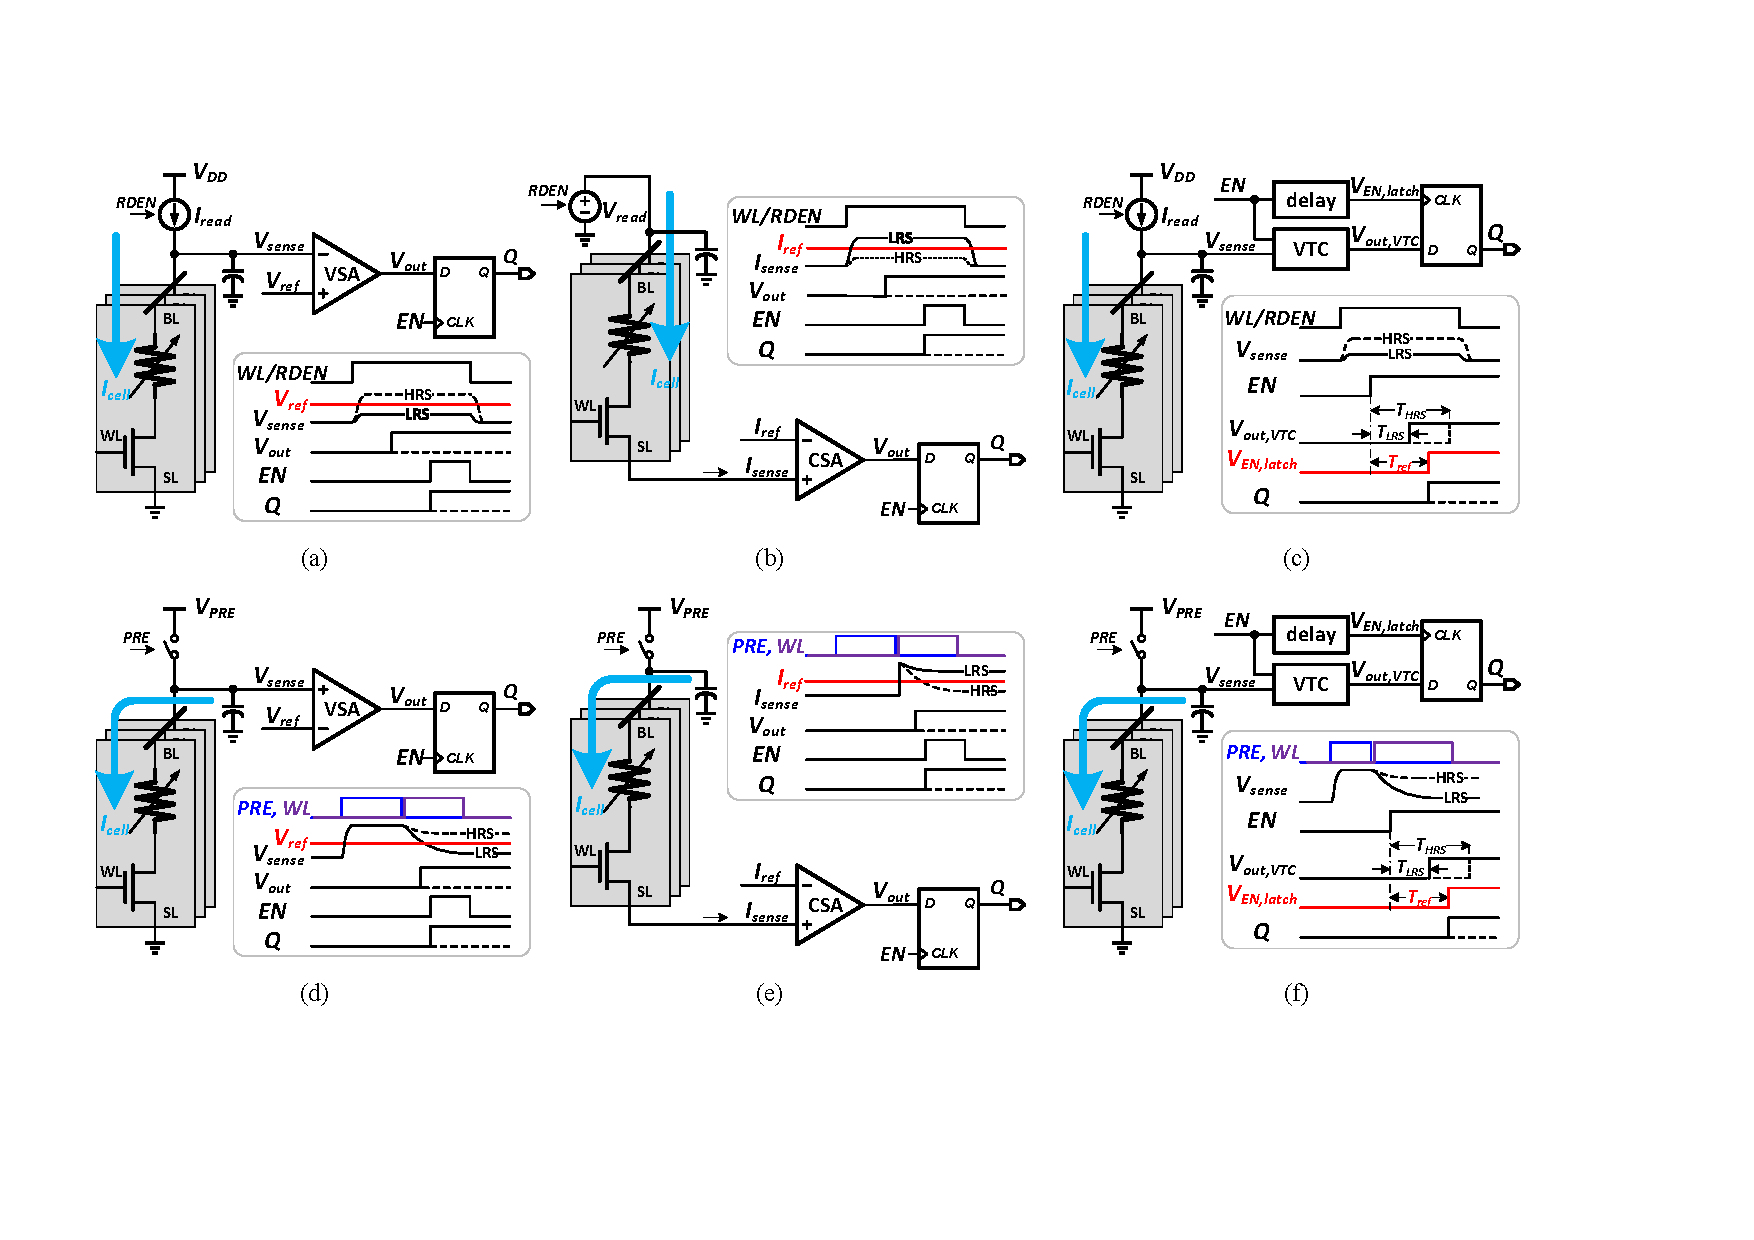
\includegraphics[width=0.95\textwidth]{fig/SA_types_new2.pdf}}
\caption{
The basic conceptual circuit schematics of three different sensing schemes for NVM array: (a) Voltage mode, (b) Current mode, and (c) Time mode w/o precharge process and (d) - (f) the above-mentioned sensing schemes w/ precharge process. 
Assuming one specific bitcell is selected.
}
\label{fig_sensing_mode}
\end{figure*}

\subsection{Prior Sensing Schemes of RRAM}

RRAM sensing is to convert the resistance state of the accessed RRAM bitcell into a digital value.
Because of the typical single-ended access operation, RRAM sensing schemes are different from conventional SRAM sensing but similar to DRAM sensing. 
% \st{Thanks to the feature of non-destructive reading under a reasonable read voltage, the sensing approaches of RRAM array are more flexible than that of conventional DRAM array.} 
Fig \ref{fig_sensing_mode} illustrates the operation principles of three main sensing modes (i.e., voltage mode, current mode, and time mode).

\subsubsection{Voltage Mode Sensing}
In the voltage mode sensing schemes \cite{yang20132mb, chang201419}, the bitcell voltage is sensed and compared with a reference voltage, which is a median value of an HRS cell and an LRS cell.
Fig. \ref{fig_sensing_mode}(a) illustrates the basic conceptual schematic of the voltage mode sensing for RRAM. The data stored in the bitcell is retrieved by forcing a fixed read current $I_{read}$ to the bit line (BL), and sensing the bit line voltage $V_{BL}$ by a voltage mode sense amplifier (VSA). 

\subsubsection{Current Mode Sensing} In the current mode sensing  \cite{jain201913, lo2018reram} (Fig. \ref{fig_sensing_mode}(b)), the data stored in the bitcell is retrieved by forcing a small fixed read voltage $V_{read}$ (smaller than the programming voltage so that the cell's state is not disturbed) to BL, and the 
%read current $I_{read}$ from source line is mirrored to compare
current through the bitcell is sensed and compared with a reference current $I_{ref}$ by a current mode sense amplifier (CSA). The reference current could be generated by two replica columns directly or by an extra reference generator circuit.

\subsubsection{Time Mode Sensing} Fig. \ref{fig_sensing_mode}(c) shows the operation of the time mode sensing \cite{trinh2018time}. 
The bitline voltage is converted into the time domain by a voltage-to-time converter (VTC) in the format of a long/short delay. A D-type flip-flop (DFF) serves as a time domain sense amplifier to compare the VTC result with an intrinsic delay that acts as a time domain reference. 
Once the enable signal $EN$ is activated, the VTC generates a signal $V_{out,VTC}$ with a time delay, depending on the input voltage $V_{sense}$, as illustrated in the timing diagram in Fig. \ref{fig_sensing_mode}(c). More specifically, an RRAM bitcell in LRS (HRS) determines a low (high) sense voltage $V_{sense}$, which generates a short (long) time delay $T_{LRS}$ ($T_{HRS}$) when a non-inverting VTC is assumed. The delay difference reflects the bitcell state, which is discriminated by the following DFF. Meanwhile, the enable signal generates a delayed signal $V_{EN,latch}$ by a delay chain with a fixed delay time $T_{ref}$ as the time domain reference, which is intermediate between $T_{LRS}$ and $T_{HRS}$. If the bitcell is in the LRS (HRS) state, the transition of $V_{out,VTC}$ will occur at $T_{LRS}<T_{ref}$ ($T_{HRS}>T_{ref}$), hence the latch will capture the high (low) logic level. As a result, the latch output indicates the bitcell state. 
% Ideally, the transition of $V_{EN,latch}$ occurs at $t_{ref}=$

In practice, however, the read operation is divided into three different phases -- precharging, developing, and sensing. BL is precharged to a precharge voltage $V_{PRE}$ before activating the word line (WL) and then kept floating. When activating WL, BL is discharged at different speeds according to the state of the cell. This developing phase is to obtain enough sensing margin. Then, a sense amplifier is enabled to detect the state.
Fig. \ref{fig_sensing_mode}(d)-(f) illustrate the above-mentioned three types of sensing schemes, where the current through the selected bitcell $I_{cell}$ is the discharge current drawing from the parasitic capacitor of bitline $C_{BL}$. The read energy can be reduced by precharging BL because the energy is only dissipated for charging the parasitic capacitor $C_{BL}$. While without precharging, the selected bitcell consumes extra energy as well during WL is activated.
% \textcolor{red}{Is it really necessary to precharge before sensing for NVM? YES!}

It should be noted that a latch (usually DFF) is necessary to hold the read-out value until the next read operation. This latch is usually driven by a read clock signal. For the time mode sensing, the DFF also acts as a sense amplifier, which compares the time delay of input signal $D$ and clock signal $CLK$.
Besides, an absolute reference voltage or current is required for voltage or current mode sensing while the time mode sensing is reference-less, simplifying the peripheral circuit design.
 As a result, the time mode sensing saves considerable area overhead compared with the conventional voltage mode and current mode sensing schemes.

\begin{figure}[!t]
\centerline
{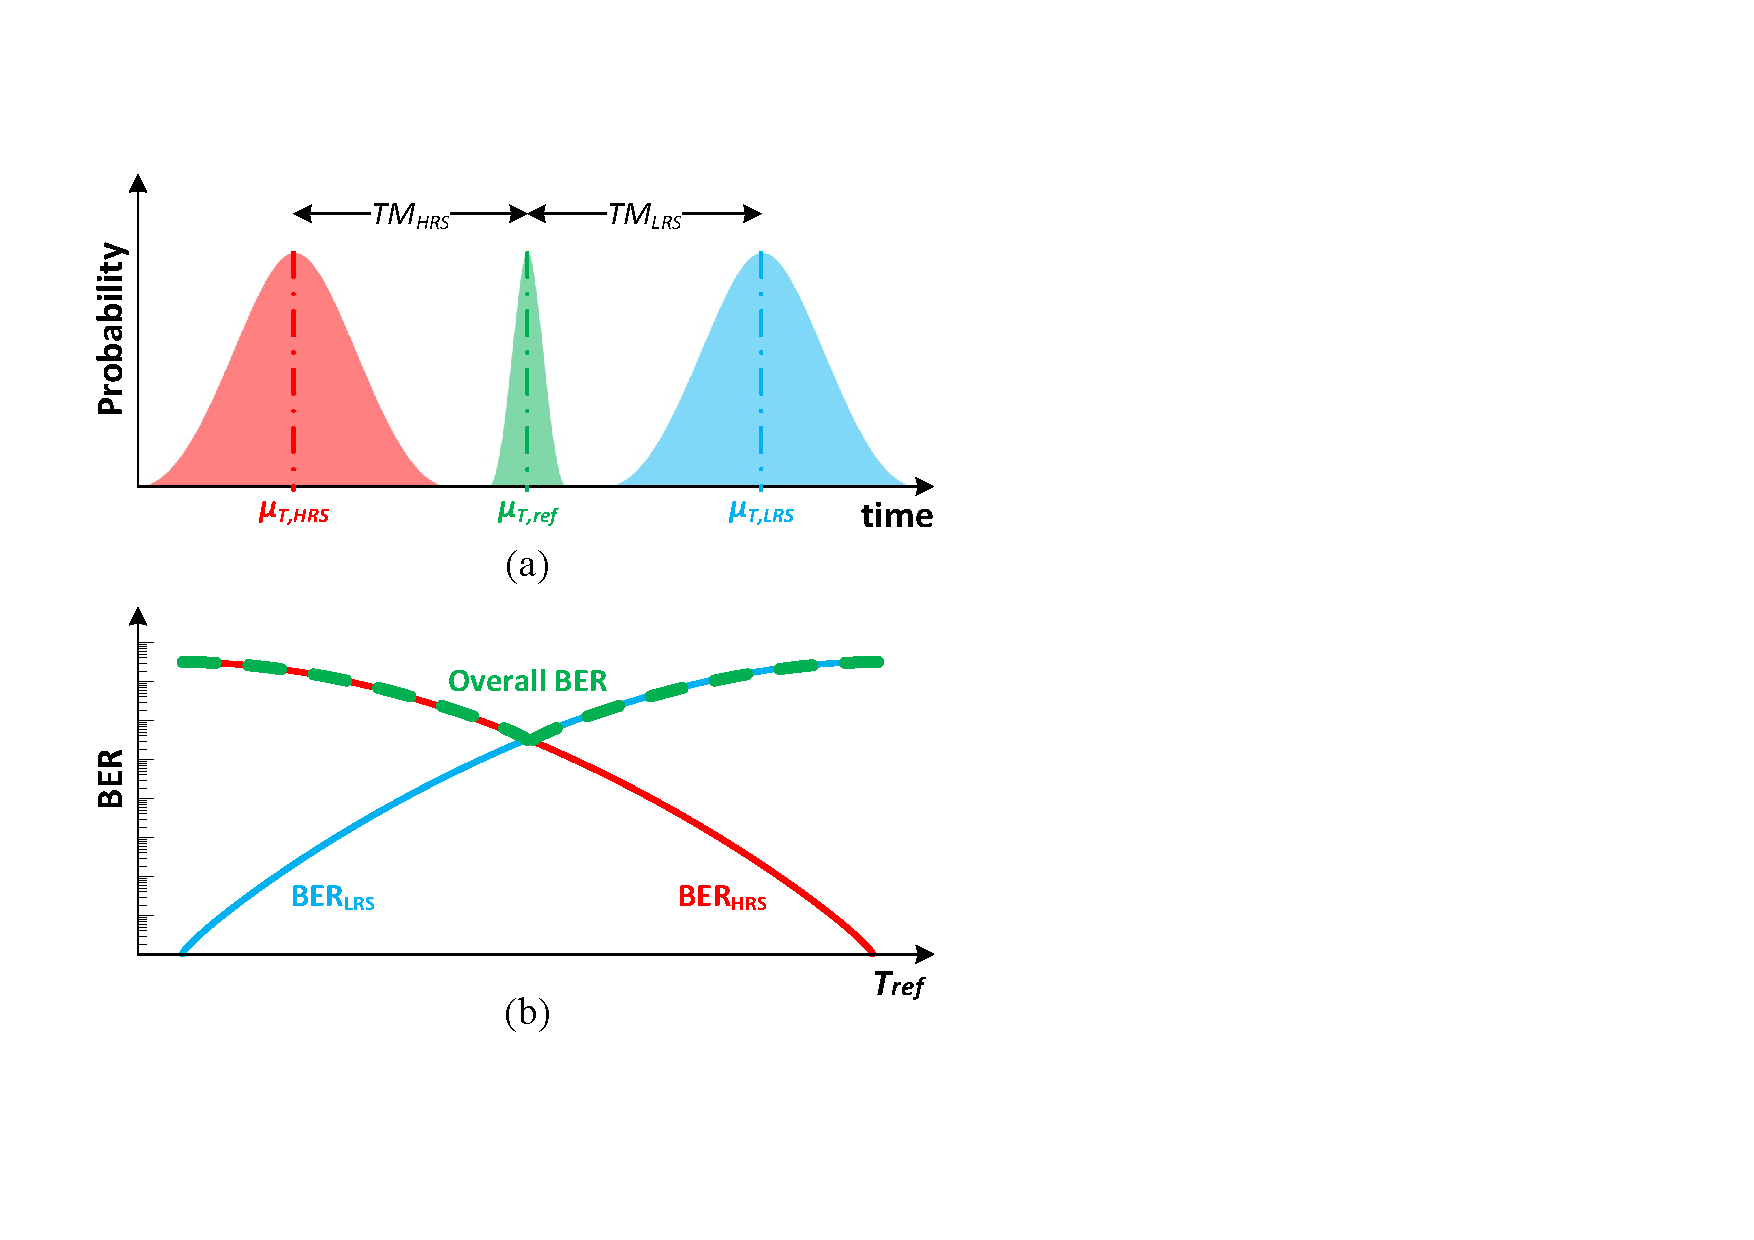
\includegraphics[width=0.42\textwidth]{fig/BER_probability.pdf}}
\caption{(a) Probability distribution of the time delay $T_{LRS}$, $T_{HRS}$ and time margin definition. (b) BER in LRS and HRS versus reference time $T_{ref}$ and the overall BER when optimizing $T_{ref}$.}
\label{fig_BER_probability}
\end{figure}

%% figure in the next section
\begin{figure*}[!t]
\centerline
{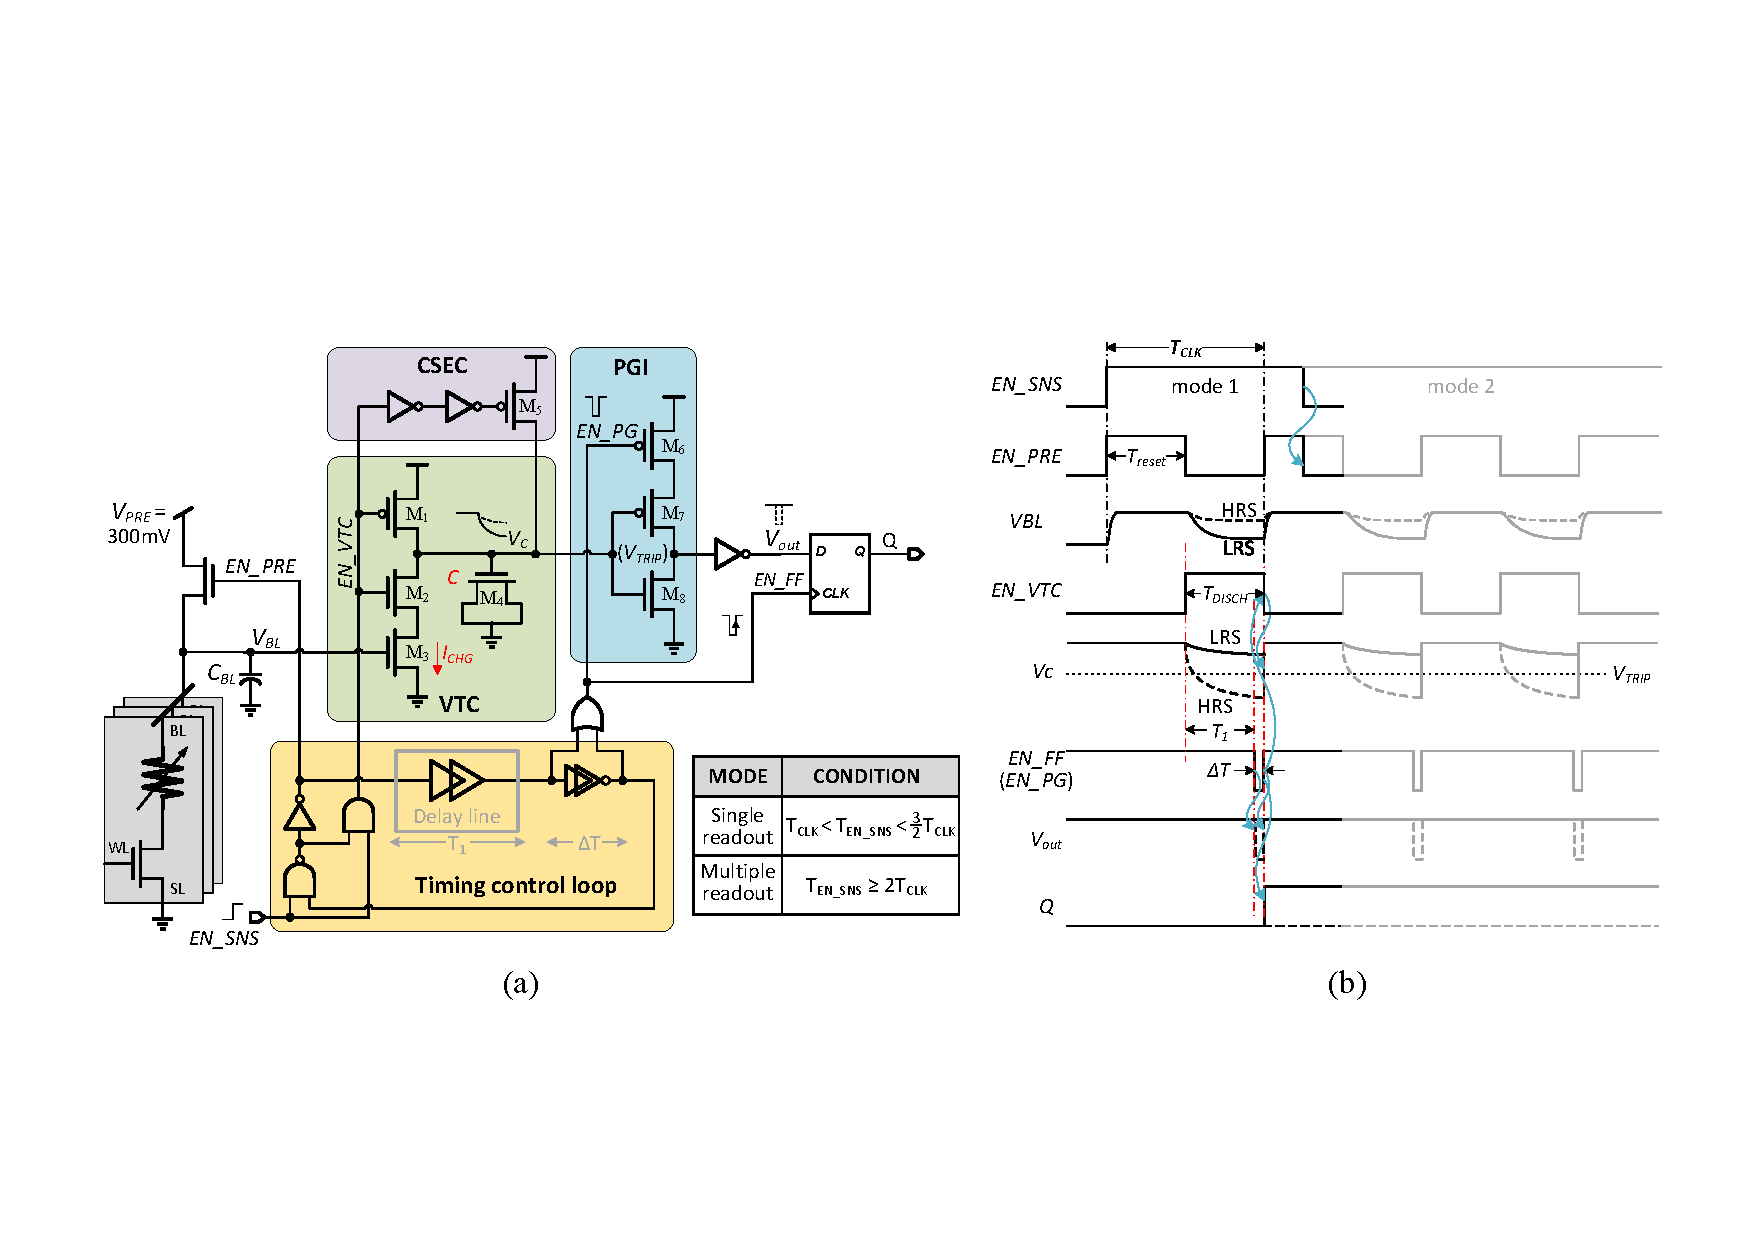
\includegraphics[width=0.97\textwidth]{fig/time_sensing_single.pdf}}
\caption{Proposed time-based single-level sensing: (a) circuit schematic that consists of voltage-time converter (VTC), power gating inverter (PGI), charge sharing-induced error compensation (CSEC) circuit, and time-domain controller. (b) Typical waveforms of critical nodes for different RRAM states (LRS and HRS) in different readout modes. }
\label{fig_prop_circuit}
\end{figure*}

\subsection{Challenges of Robust Sensing}
\label{challenges}

To enlarge the sensing margin and distinguish the resistance states reliably, higher bitline voltage $V_{BL}$ is desirable. However, the $V_{BL}$ must be kept considerably smaller than the typical program voltage to prevent read disturbance. This leads to an inevitable trade-off between read robustness and read disturbance.
Furthermore, random process variations degrade the sensing margins and increase read BER.

Fig. \ref{fig_BER_probability}(a) shows the probability distribution of the time delay at different states $T_{LRS}$ and $T_{HRS}$. 
The time domain reference $T_{ref}$ needs to be set appropriately to ensure adequate margin when variations are considered. 
Since the resistance of the RRAM is assumed to be Gaussian distributed \cite{6948806}, the time margin $TM_{LRS}=T_{LRS}-T_{ref}$ ($TM_{HRS}=T_{ref}-T_{HRS}$) can be represented as a random variable with the mean value $\mu_{TM,LRS}$ ($\mu_{TM,HRS}$) and the standard deviation $\sigma_{TM,LRS}$ ($\sigma_{TM,HRS}$). 
Ideally, the transition of $V_{EN,latch}$ occurs at $T_{ref}=\frac{1}{2}(T_{LRS}+T_{HRS})$ to maximize the time margin $TM$ ($TM=min	\left\{TM_{LRS}, TM_{HRS}\right\}$) and minimize the read BER.
Setting the reference time $T_{ref}$ away from $T_{LRS}$ will reduce $BER_{LRS}$ but increase $BER_{HRS}$, and vice versa, as illustrated in Fig. \ref{fig_BER_probability}(b).
The BER in LRS (HRS) is the probability that the time margin $TM_{LRS}$ ($TM_{HRS}$) is negative, which is given by \cite{trinh2018time}
\begin{align}
\label{eq_ber}
BER_X &= {\rm Pr}[TM_X<0] \notag \\
      &= \frac{1}{2}\left[1+{\rm erf}\left(\frac{-1/\sqrt{2}}{\sigma_{TM,X}/\mu_{TM,X}}\right)\right]
\end{align}
% \begin{align}
% \label{eq_ber}
% BER_X = Pr[TM_X<0] 
%       = \frac{1}{2}[1+erf(\frac{1}{\sqrt{2}} \frac{1}{\sigma_{TM,X}/\mu_{TM,X}})]
% \end{align}
where the subscript $X$ stands for the state of the bitcell (either LRS or HRS), and erf is the Gaussian error function \cite{walpole1993probability}. 
From \eqref{eq_ber}, the read robustness against variations depends only on the sensing margin variability $\sigma_{TM,X}/\mu_{TM,X}$.
For example, a sensing margin variability of 0.21 (0.167) leads to a BER of $10^{-6}$ ($10^{-9}$).
As expected, lower variability in the sensing margin achieves better (i.e., lower) read BER. 

The overall BER is determined by the worst case between LRS and HRS in Eq. \eqref{eq_ber}. 
The sensing margin is limited because (a) the voltage or current applied to the bitcell is small to avoid disturbing, and (b) the resistance ratio is not high enough considering variations.
It is noted that in the worst case where the LRS and HRS values are overlapped (i.e., $R_{LRS}>R_{HRS}$), the states are indistinguishable, and hence it is impossible to read the bitcell correctly. 




\section{Proposed Time-based Sensing Scheme and Theoretical Analysis}
\label{sec_prop}
To improve the robustness of reading and achieve ultra-low BER, this paper proposes a time-based sensing scheme with a built-in read control loop to support both single readout for normal application and multiple readout for massive repeated sampling.
This section describes the circuit design and detailed analysis of the proposed time-based sensing scheme.

The proposed time-based sensing circuit is depicted in Fig. \ref{fig_prop_circuit}(a), which consists of (1) a voltage-time converter (VTC) to convert the BL voltage to a time delay, (2) a power gating inverter (PGI) to minimize the short-circuit current, (3) a charge sharing-induced error compensation (CSEC) circuit to eliminate the charge sharing-induced error and improve the read margin, (4) a built-in timing control loop for different reading modes, and (5) a DFF to compare and store the state. 

A low precharge voltage ($V_{PRE}$ = 300 mV) is applied to BL through an NMOS transistor. The sensing circuit stays in the precharge (reset) phase ($V_{BL}$ = $V_{PRE}$) when the precharge enable signal $EN\_PRE$ is asserted. When $EN\_PRE$ is deasserted and a wordline is selected, $V_{BL}$ is discharged with different speeds according to the bitcell state, resulting in the development of $V_{BL}$ for sensing. During this time, the enable signal $EN\_VTC$ is activated to enable the VTC and convert the bitline voltage $V_{BL}$ to the time delay signal. The capacitor node voltage $V_C$ is initially precharged to $V_{DD}$ when the enable signal $EN\_VTC$ is low. The signal $EN\_VTC$ is activated when the sensing phase begins, and the capacitor node voltage $V_C$ is discharged by the current $I_{DISCH}$, which is inversely proportional to $V_{BL}$. The discharge voltage $V_C$ is, thereafter, shaped by a cascaded inverter to regenerate a sharp-edge signal $V_{out}$, which reflects the bitcell state indirectly. 
Both enable signals $EN\_PRE$ and $EN\_VTC$ are generated by the sensing enable signal  $EN\_SNS$ and the timing control loop. 
Fig. \ref{fig_prop_circuit}(b) illustrates the waveforms of the critical nodes for different RRAM states in different readout modes, where the solid and dashed lines represent the RRAM in LRS and HRS, respectively.
We will analyze the design details of each block in the following subsections.


\subsection{Voltage-to-Time Converter (VTC)}
The basic principle of VTC designs is to charge (or discharge) a capacitor from its initial voltage to a certain level and subsequently detect the time when the voltage across the capacitor crosses the threshold voltage. The ramp-based VTC generates a fixed ramp using a constant current source integrated over a capacitor and compares the ramp with the input-controlled threshold voltage \cite{naraghi20109,weng2016continuous}. The current-starved-inverter (CSI) based VTC generates the current controlled by the applied input signal and compares the voltage across the capacitor with a fixed threshold voltage \cite{zhu2016skew,chen20140,macpherson20135gs}.
Among these architectures, the CSI-based VTC topology is compact and suitable for high-speed applications \cite{macpherson20135gs}.

This work employs the CSI-based VTC structure to convert the bitline voltage into a pulse delay, considering its low power consumption, high speed, and small silicon area overhead.  
As shown in Fig. \ref{fig_prop_circuit}, when the enable signal $EN\_VTC$ is low, M$_1$ resets the capacitor node $V_C$ to $V_{DD}$; when $EN\_VTC$ is high, M$_3$ starts to discharge $V_C$ with a current $I_{DISCH}$ controlled by the bitline voltage $V_{BL}$. 
When the VTC receives a rising transition in $EN\_VTC$, it discharges the capacitor node $V_C$ and exhibits a gate delay expressed as
\begin{align}
\label{eq_delay}
T_{delay} &= C\frac{V_{DD}-V_{TRIP}}{I_{DISCH}}
\end{align}
where $V_{DD}$ is the supply voltage, $V_{TRIP}$ is the trip voltage of the subsequent inverter, $C$ is the total capacitor at the node $V_C$ (including MOS capacitance and parasitic capacitance), and $I_{DISCH}$ is the current delivered by the pull-down network of the CSI. $I_{DISCH}$ is essentially equal to the current delivered by $M_3$, reflecting the bitline voltage $V_{BL}$. 

\begin{figure}[!t]
\centerline
{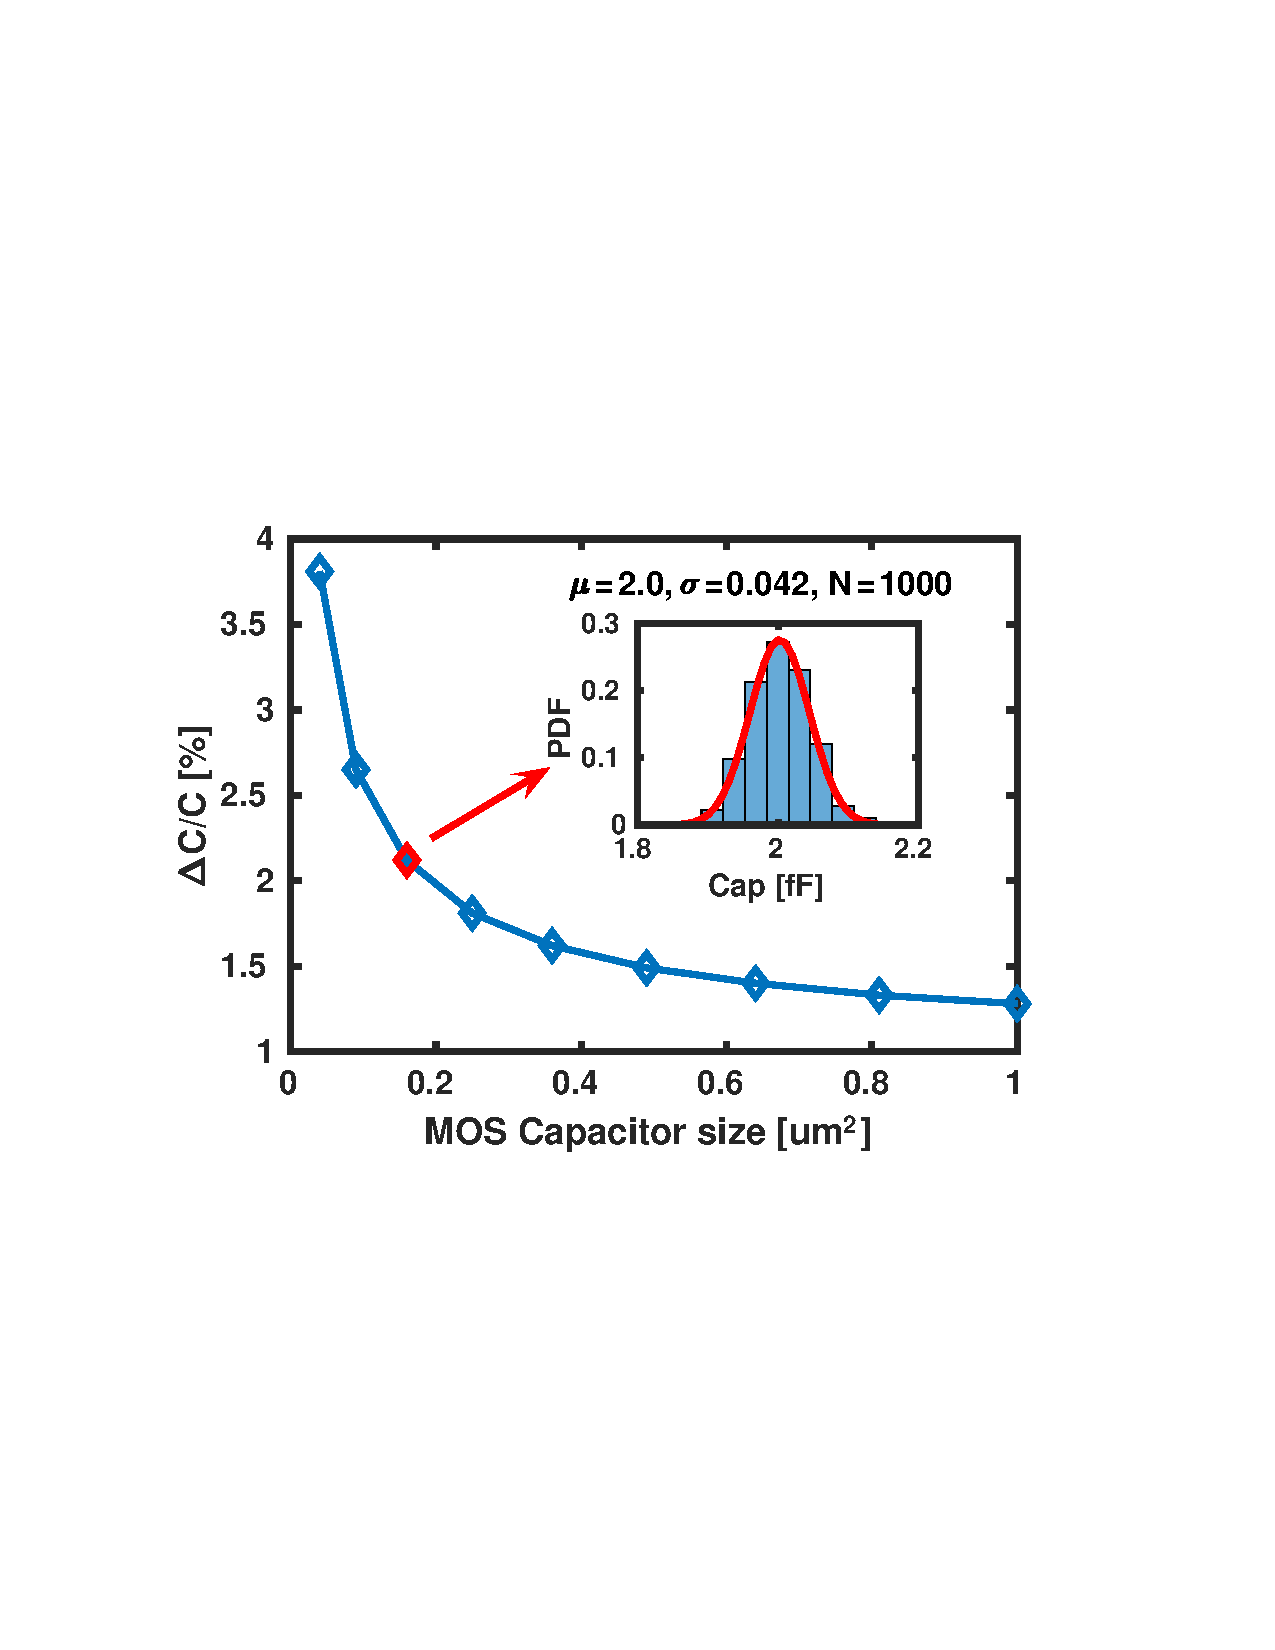
\includegraphics[width=0.46\textwidth]{fig/moscap.pdf}}
\caption{MOS capacitor mismatch for different capacitor sizes and the capacitor distribution when the MOS size is $W \times L=0.16~\rm \micro m^2$.}
\label{fig_moscap}
\end{figure}

One important trade-off in the area comes from the MOS capacitor -- a large capacitor minimizes the discharge time variations caused by mismatch at the cost of area overhead. Monte Carlo (MC) simulations with device mismatches and process variations are presented in Fig. \ref{fig_moscap}. In our design, the MOS capacitor size is selected as $W \times L=0.16~\rm \micro m^2$, resulting in a mean capacitance value of $2~\rm fF$ and a standard deviation of $42~\rm aF$. The normalized variance of capacitor is $\Delta C/C = 2.1\%$.
% \textcolor{blue}{Compared with other parts, the capacitor variation is small, }
SPICE simulations show that it is a good balance between performance and area. 

Since $V_{BL}$ is limited to the precharge voltage ($V_{PRE}$=300 mV), it is necessary to increase the size of the pull-down transistor M$_3$ to distinguish the current in different states and attenuate the effect of mismatch. As a result, the parasitic capacitance at the drain of M$_3$ is not negligible, leading to charge sharing-induced error at the transition of $EN\_VTC$. We will explain and address this issue in detail next.

\subsection{Charge Sharing-induced Error Compensation (CSEC)}

\begin{figure}[!t]
\centerline
{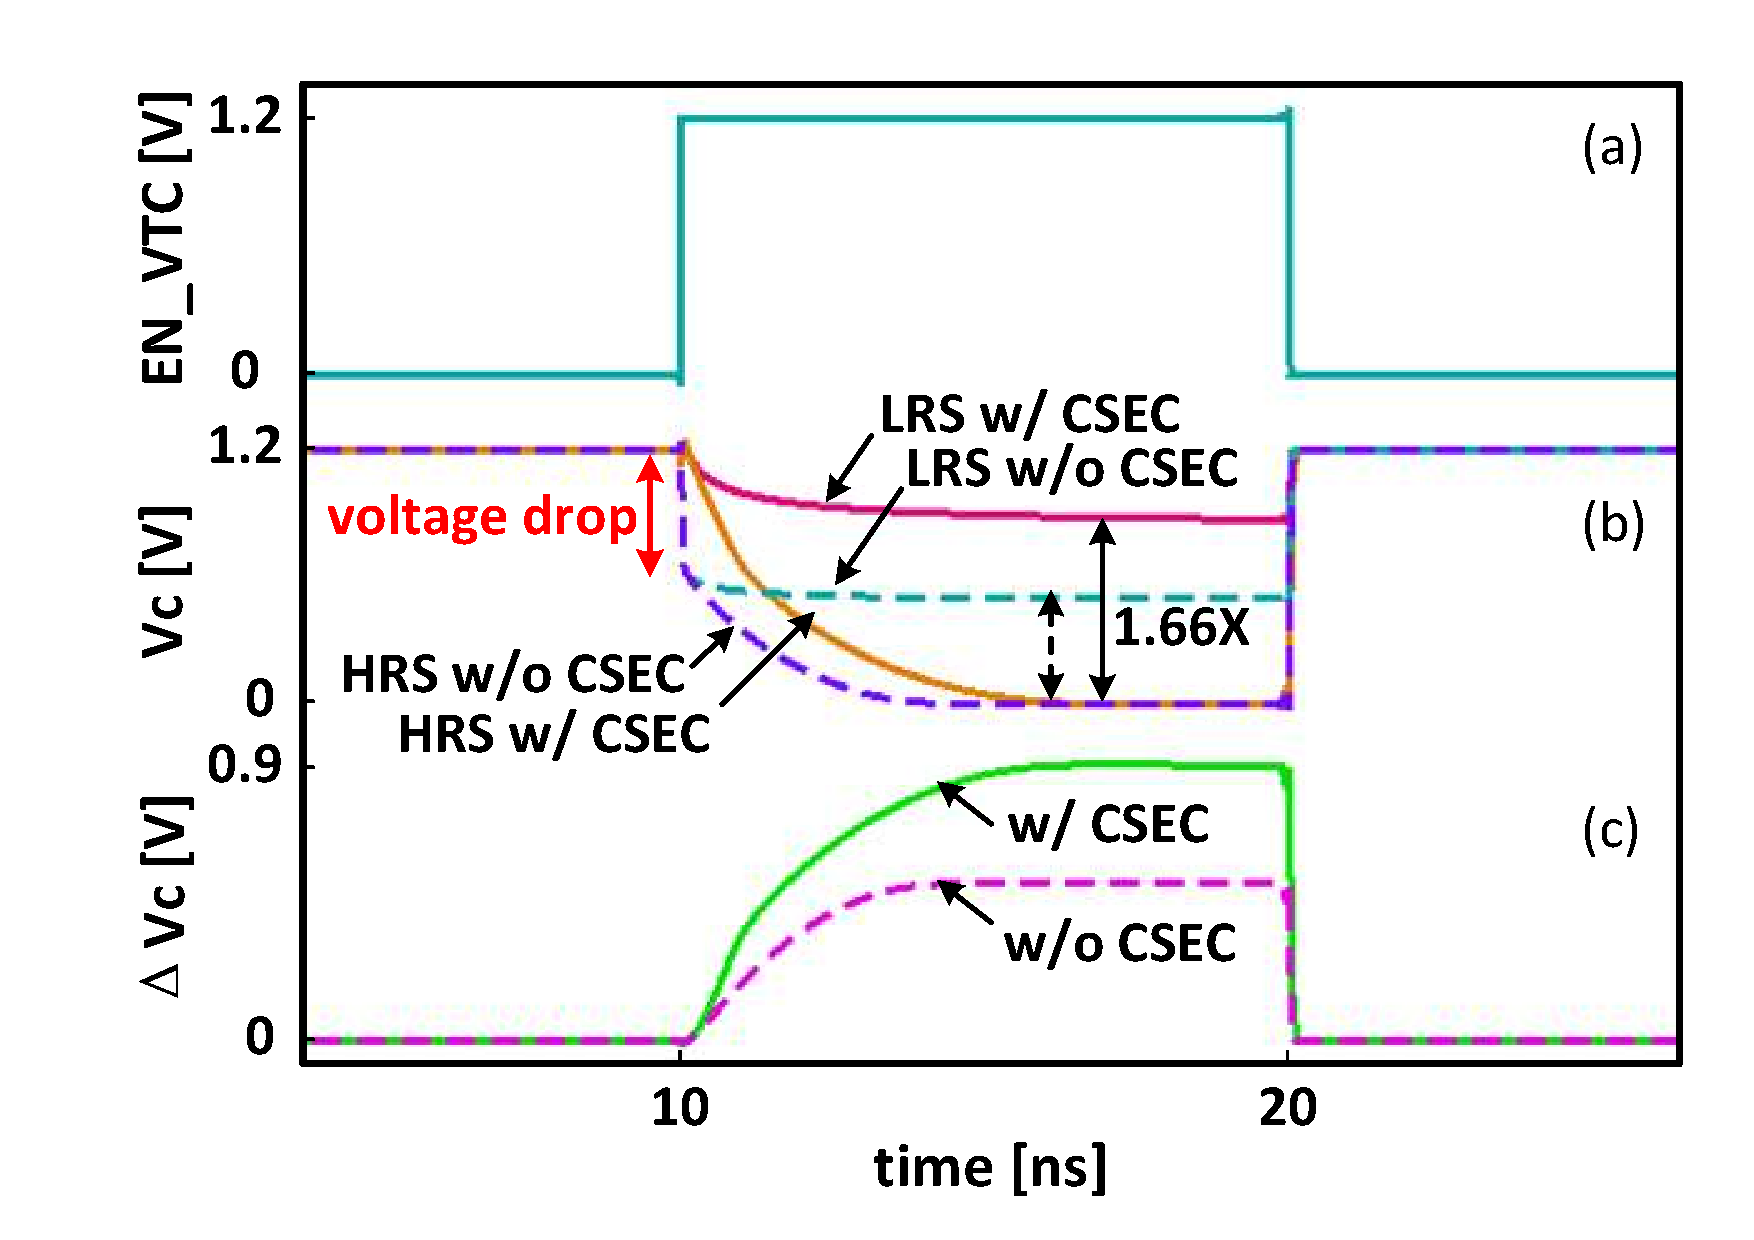
\includegraphics[width=0.48\textwidth]{fig/waveform_CIEF.pdf}}
\caption{
Voltage margin with and without CSEC in a typical case. (a) Voltage to time conversion enable signal $EN\_VTC$; (b) The capacitor node voltage $V_C$ without CSEC (dashed lines) and with CSEC (solid lines); and (c) The voltage difference of $V_C$ when RRAM is in LRS and HRS ($\Delta V_C = V_C(LRS) - V_C(HRS)$). The voltage margin increases 1.66 times with CSEC circuit.
}
\label{fig_CIEF}
\end{figure}

When the enable signal $EN\_VTC$ is inactive, the capacitor node voltage $V_C$ is charged to $V_{DD}$ by the PMOS M$_1$ while the drain voltage of M$_3$ keeps zero because of the pull-down current of M$_3$. At the time of the transition of signal $EN\_VTC$, M$_2$ turns on and draws a high transient current from the node $V_C$ to charge the drain of M$_3$. This leads to a sharp voltage drop of $V_C$ because the pull-up transistor M$_1$ is turned off and the charges stored in the MOS capacitor M$_4$ are shared with the drain capacitor of M$_3$ and the source capacitor of M$_2$. 
The charge sharing-induced voltage drop shrinks the voltage margin for HRS and LRS, and hence risks incorrect sensing and increases the read BER, as the dashed lines are shown in Fig. \ref{fig_CIEF}. 
This charge sharing-induced error is severer when the size of M$_3$ is large considering the large parasitic capacitor at the drain of M$_3$.
% shrinking memory window

Avoiding the charge sharing-induced error benefits robust and accurate sensing by widening the margin of capacitor node voltage $V_C$ in different resistance states (i.e., HRS and LRS).
A charge sharing-induced error compensation (CSEC) scheme is proposed to compensate for the charge and eliminate the voltage drop of $V_C$, as shown in Fig. \ref{fig_prop_circuit}. The two inverters provide a short propagation delay. Driven by the signal that is delayed by $EN\_VTC$, M$_5$ provides an extra charge current at the beginning of the signal $EN\_VTC$ goes high. As a result, the $V_C$ keeps $V_{DD}$ and holds the charge during the transition of $EN\_VTC$. 
It is to be noted that the size of $M_5$ should match the size of $M_4$ to balance the pull-up and pull-down currents for proper charge compensation. If the size of $M_5$ is too small, the voltage drop cannot be compensated completely. On the contrary, an overshoot voltage appears at the rising edge of {EN\_VTC} if the size of $M_5$ is too large.

The comparison of the discharge voltage $V_C$ in different resistance states is shown in Fig. \ref{fig_CIEF}. A 1.66$\times$ voltage margin is achieved with the proposed CSEC circuit. The enlarged sensing window can accommodate wider variations arising from the RRAM devices and other parts of the sensing circuit, improving the read reliability and reducing the read BER.   
Avoiding the charge sharing-induced error is beneficial not only to voltage margin improvement but also to energy saving for the subsequent shaping inverter. That is because $V_C$ in LRS (see Fig. \ref{fig_CIEF}) is much closer to the trip voltage of the following inverter if without CSEC, consuming a large short-circuit current during the sensing period.

\begin{figure}[!t]
\centerline
{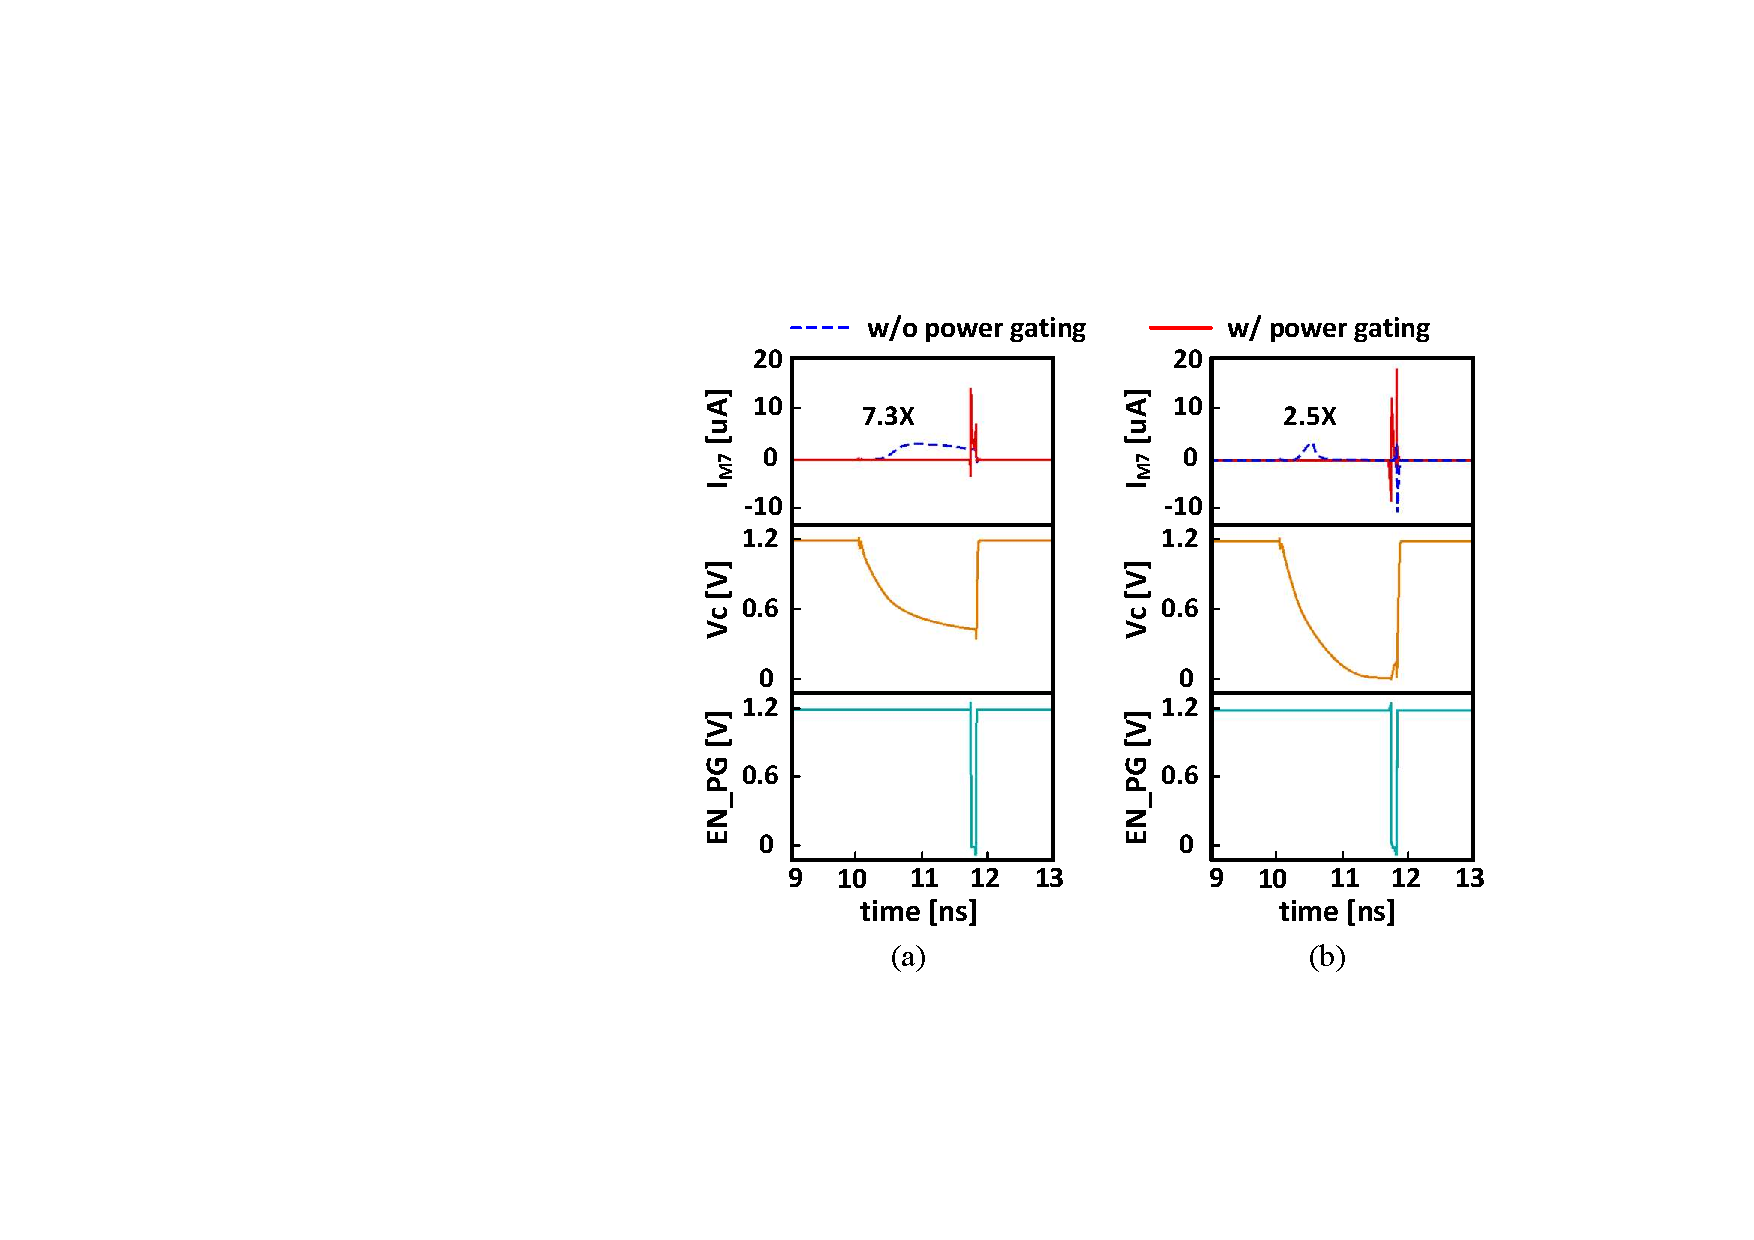
\includegraphics[width=0.5\textwidth]{fig/power_gating_current.pdf}}
\caption{Comparison of the current consumption of the shaping inverter with and without power gating. (a) $V_C$ is around $V_{DD}/2$. (b) $V_C$ is close to zero.}
\label{fig_powergating}
\end{figure}


\subsection{Power Gating Technique}
The inverter (M$_7$ and M$_8$) after VTC behaves as a voltage detector and signal shaper. The trip voltage $V_{TRIP}$ of this inverter is compared with the output of the VTC. As a result, the slow-edged capacitor node voltage $V_C$ is shaped by the cascaded inverters to generate a sharp-edged signal $V_{out}$ at the input of the subsequent DFF.

The energy drawn by the shaping inverter $E_{shaping}$ is dominated by its short-circuit current associated with the slow transition of the discharge voltage $V_C$, as determined by the operation of M$_3$ in the sub-threshold region (see Fig. \ref{fig_prop_circuit}(a)).
By inserting a PMOS sleep transistor M$_6$, the power gating inverter (PGI) is enabled only when the gate signal of M$_6$ is activated.
The gate signal $EN\_PG$ is generated directly by the combination logic from  the timing control loop. $EN\_PG$ is low active for the PGI and its positive edge triggers the DFF (see Fig. \ref{fig_prop_circuit}).
The value of $V_C$ depends on the discharge current $I_{DISCH}$ (determined by the size of $M_3$ for the same $V_{BL}$) and the discharge time $T_{DISCH}$. A short period of short-circuit current is consumed only when $EN\_PG$ is enabled and $V_C$ is close to the trip voltage of the shaping inverter (i.e., around $V_{DD}/2$). It can achieve short-circuit-current-free if $EN\_PG$ is enabled when $V_C$ is much less than the threshold voltage of M$_8$ (i.e., close to zero). 
% but with the penalty of longer sensing time. 

Fig. \ref{fig_powergating} illustrates the transition of the discharge voltage $V_C$ and the current consumption with and without power gating. 
We can see the power gating achieves $7.3\times$ and $2.5\times$ energy saving for the case of $V_C$ around $V_{DD}/2$ and zero, respectively. 
% $V_C$ is modulated by size of $M_3$.
To shape the voltage $V_C$ into a sharp edge signal at the input of the DFF, \cite{trinh2018time} adopted a $4\times$ minimum-sized inverter, resulting in a large shaping current ($\approx 50~\rm \micro A$ averaging). In this work, two cascaded inverters are used to shape the voltage and make the sensing margin positive (i.e., LRS of RRAM results in output high). By this, minimum-sized transistors are used in the PGI with the average current less than $5~\rm \micro A$ during sensing. 
The transient current spikes are caused by gate tunneling leakage when the gate voltage goes high, which is negligible compared to the shaping power. 
% Avoiding the short-circuit current is beneficial to not only power consumption but also phase linearity.

\subsection{Dual-mode Timing Controller}

% \begin{figure}[!t]
% \centerline
% {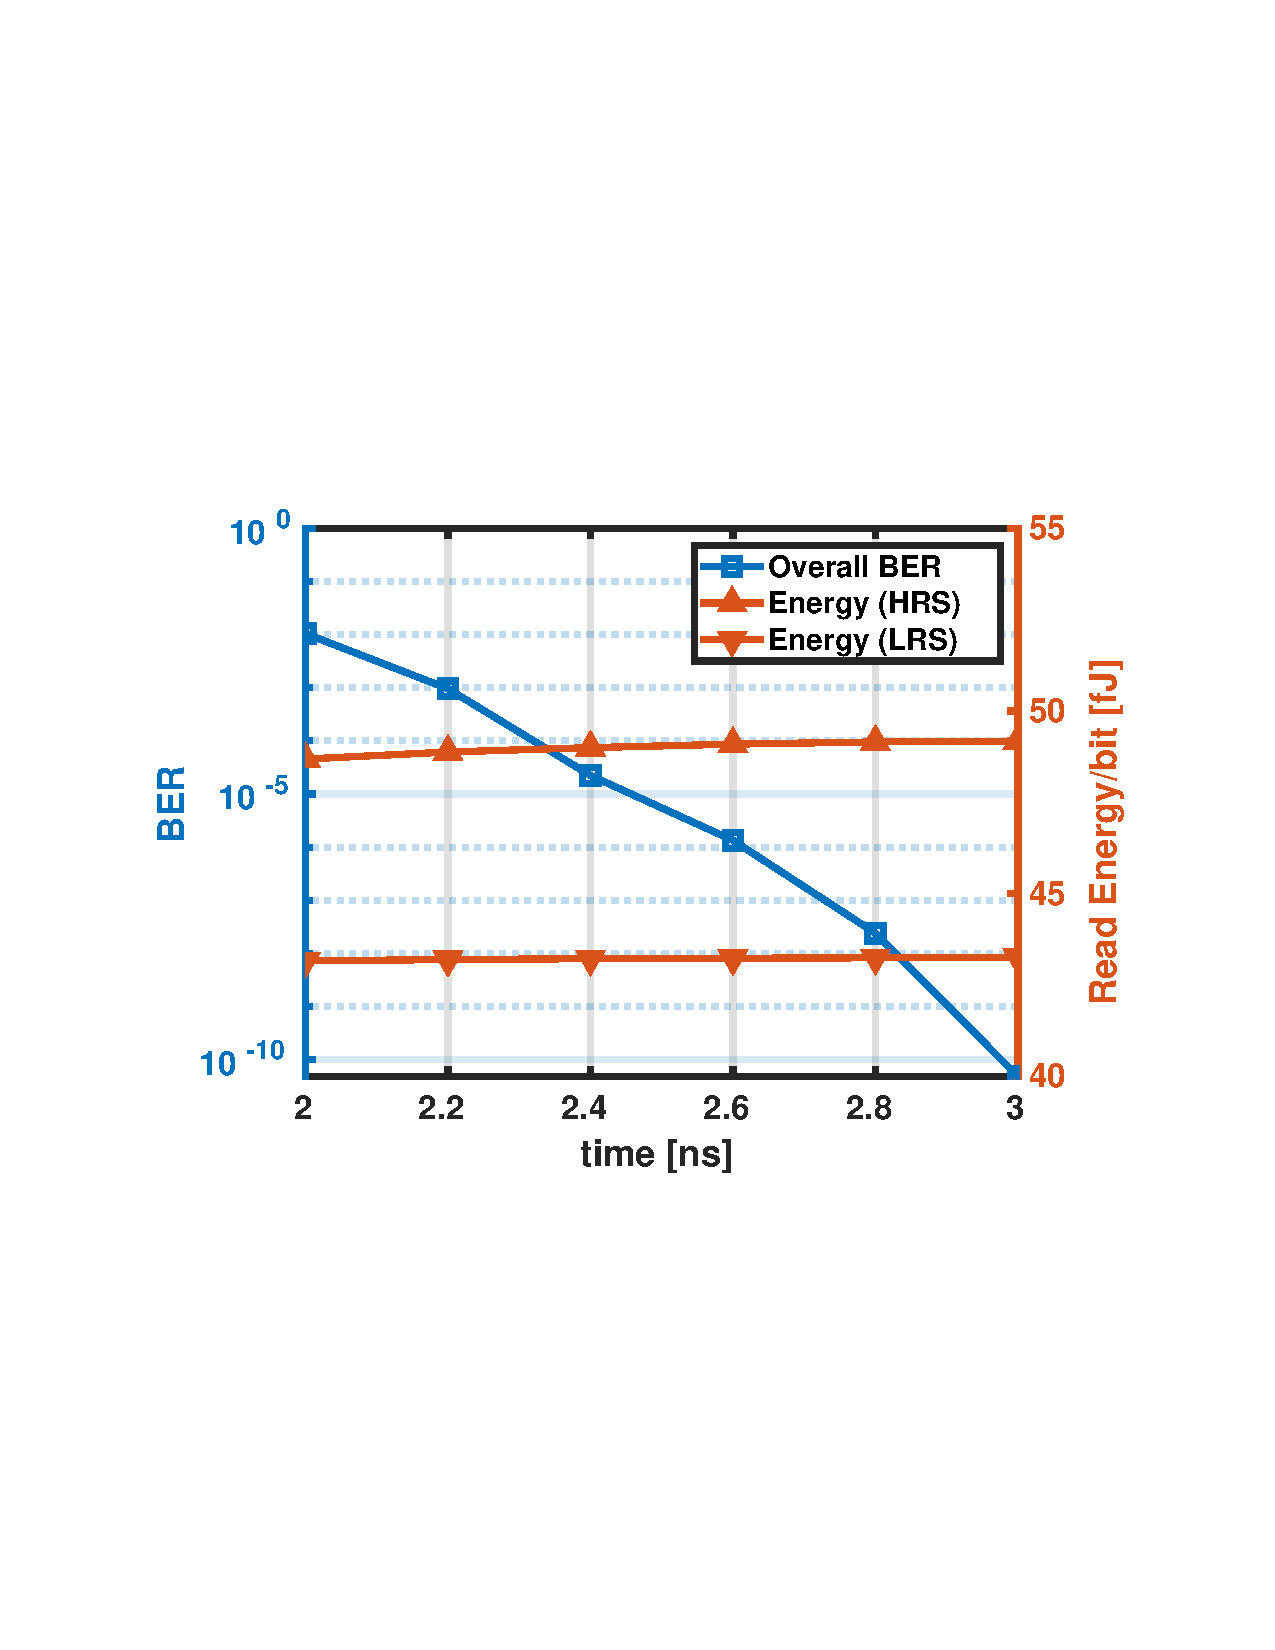
\includegraphics[width=0.45\textwidth]{fig/ber_delay_energy.pdf}}
% \caption{BER and read energy per bit of the proposed time-based sensing with respect to the delay time $T_1$.}
% \label{fig_ber_delay}
% \end{figure}

\begin{figure}[!t]
    \centering
    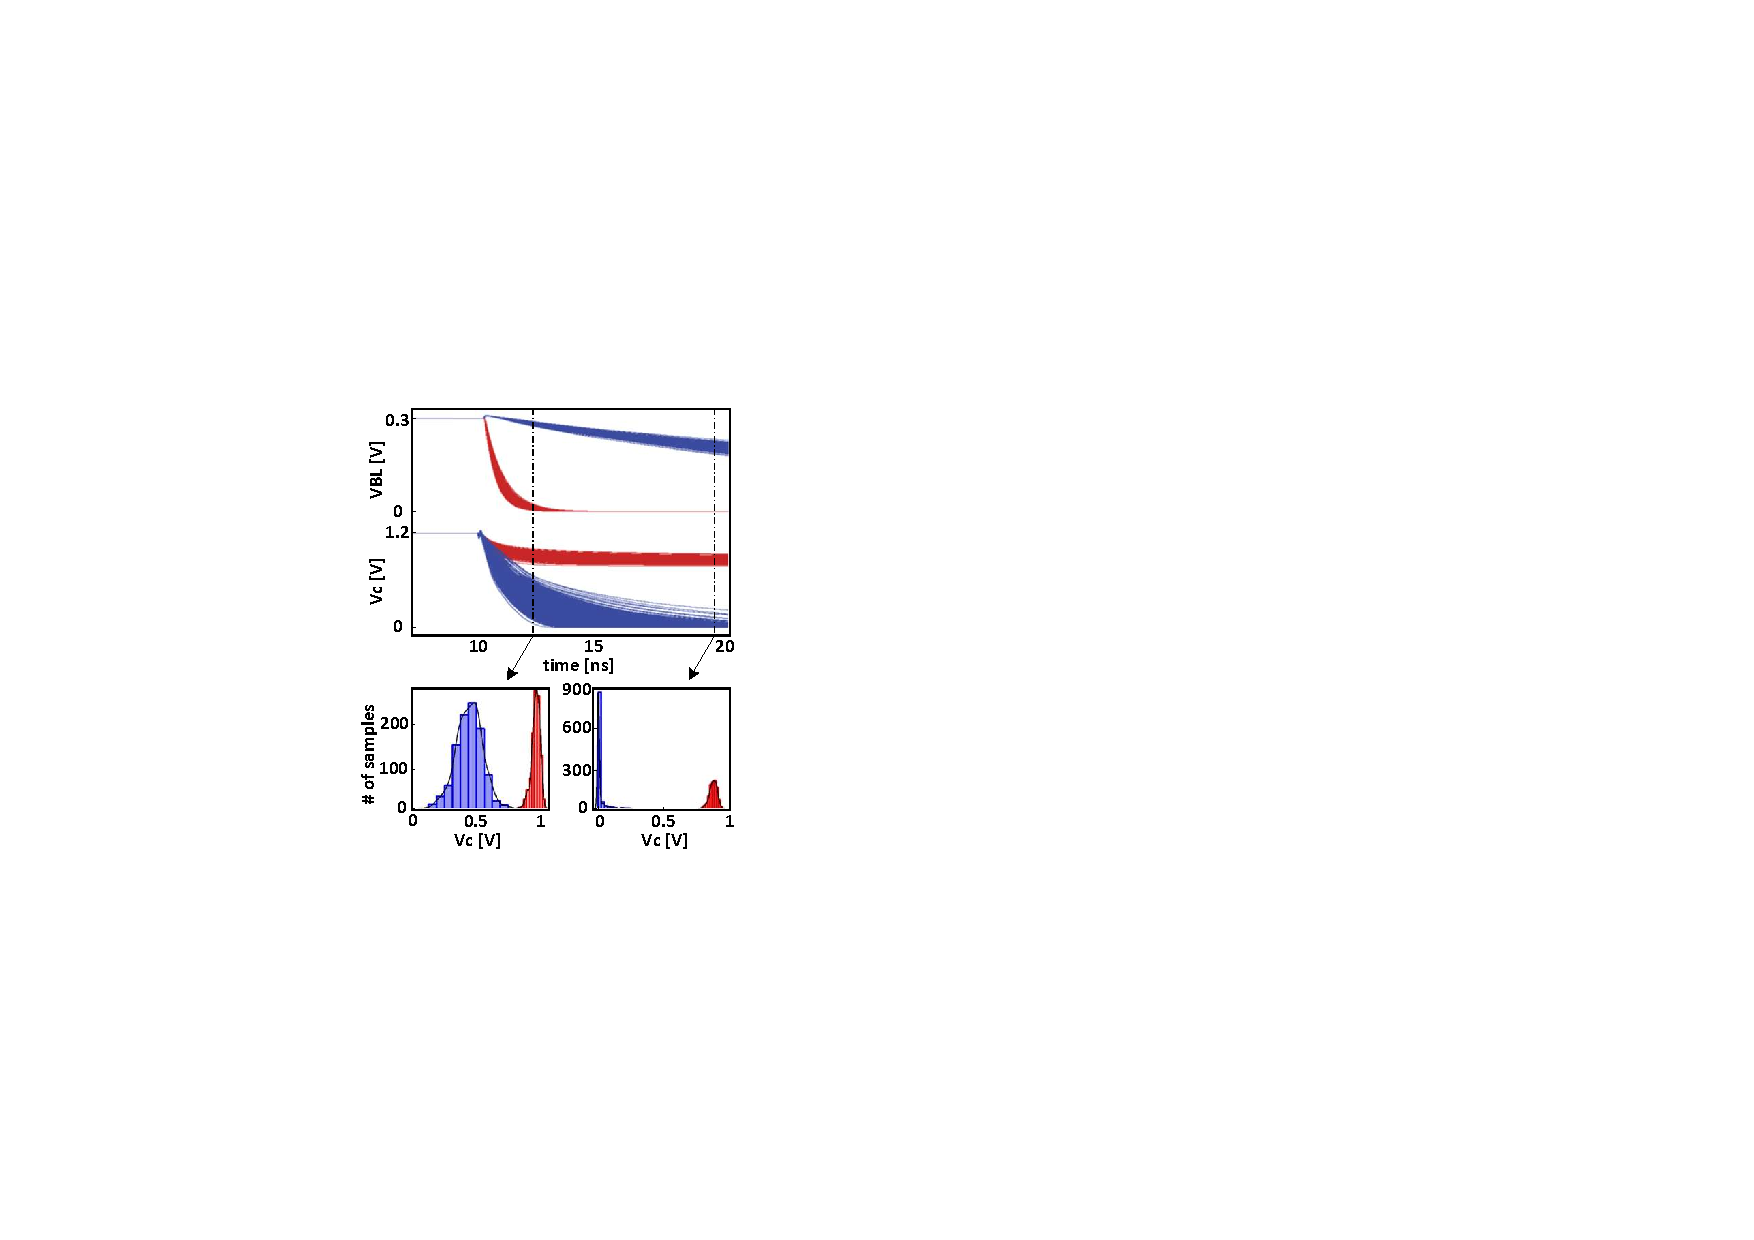
\includegraphics[width=0.4\textwidth]{fig/VC_MC_new.pdf}
    \caption{Monte Carlo simulation of $V_{BL}$ and $V_C$ in different RRAM states generated from 1000 runs. Transient waveforms (top panel) and histogram of $V_C$ at two different times (bottom panel).}
    \label{fig_vc}
\end{figure}
     
\begin{figure}[!t]
    \centering
    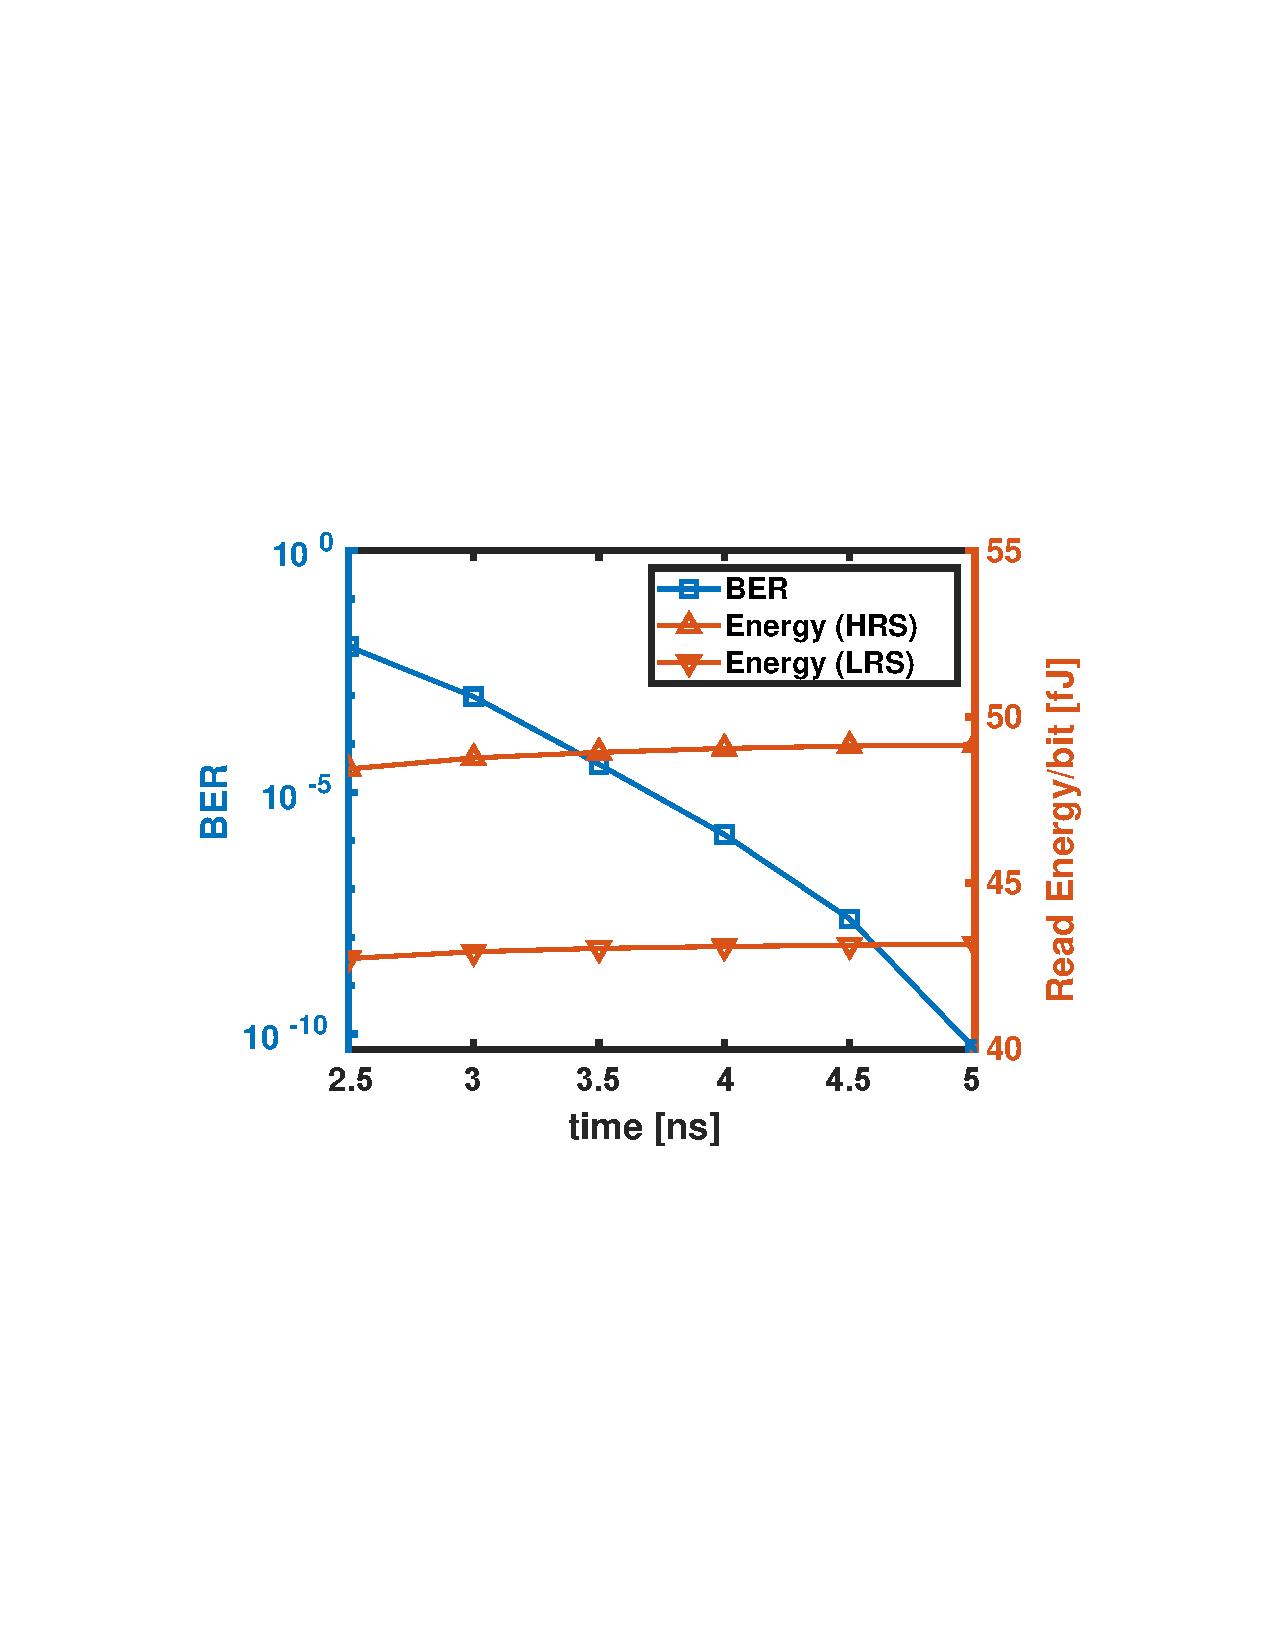
\includegraphics[width=0.45\textwidth]{fig/ber_delay_energy_new.pdf}
    \caption{
    BER and read energy per bit of the proposed time-based sensing with respect to the delay time $T_1$.}
    \label{fig_ber_delay}
\end{figure}


%% figure in the next section
\begin{figure*}[!t]
\centerline
{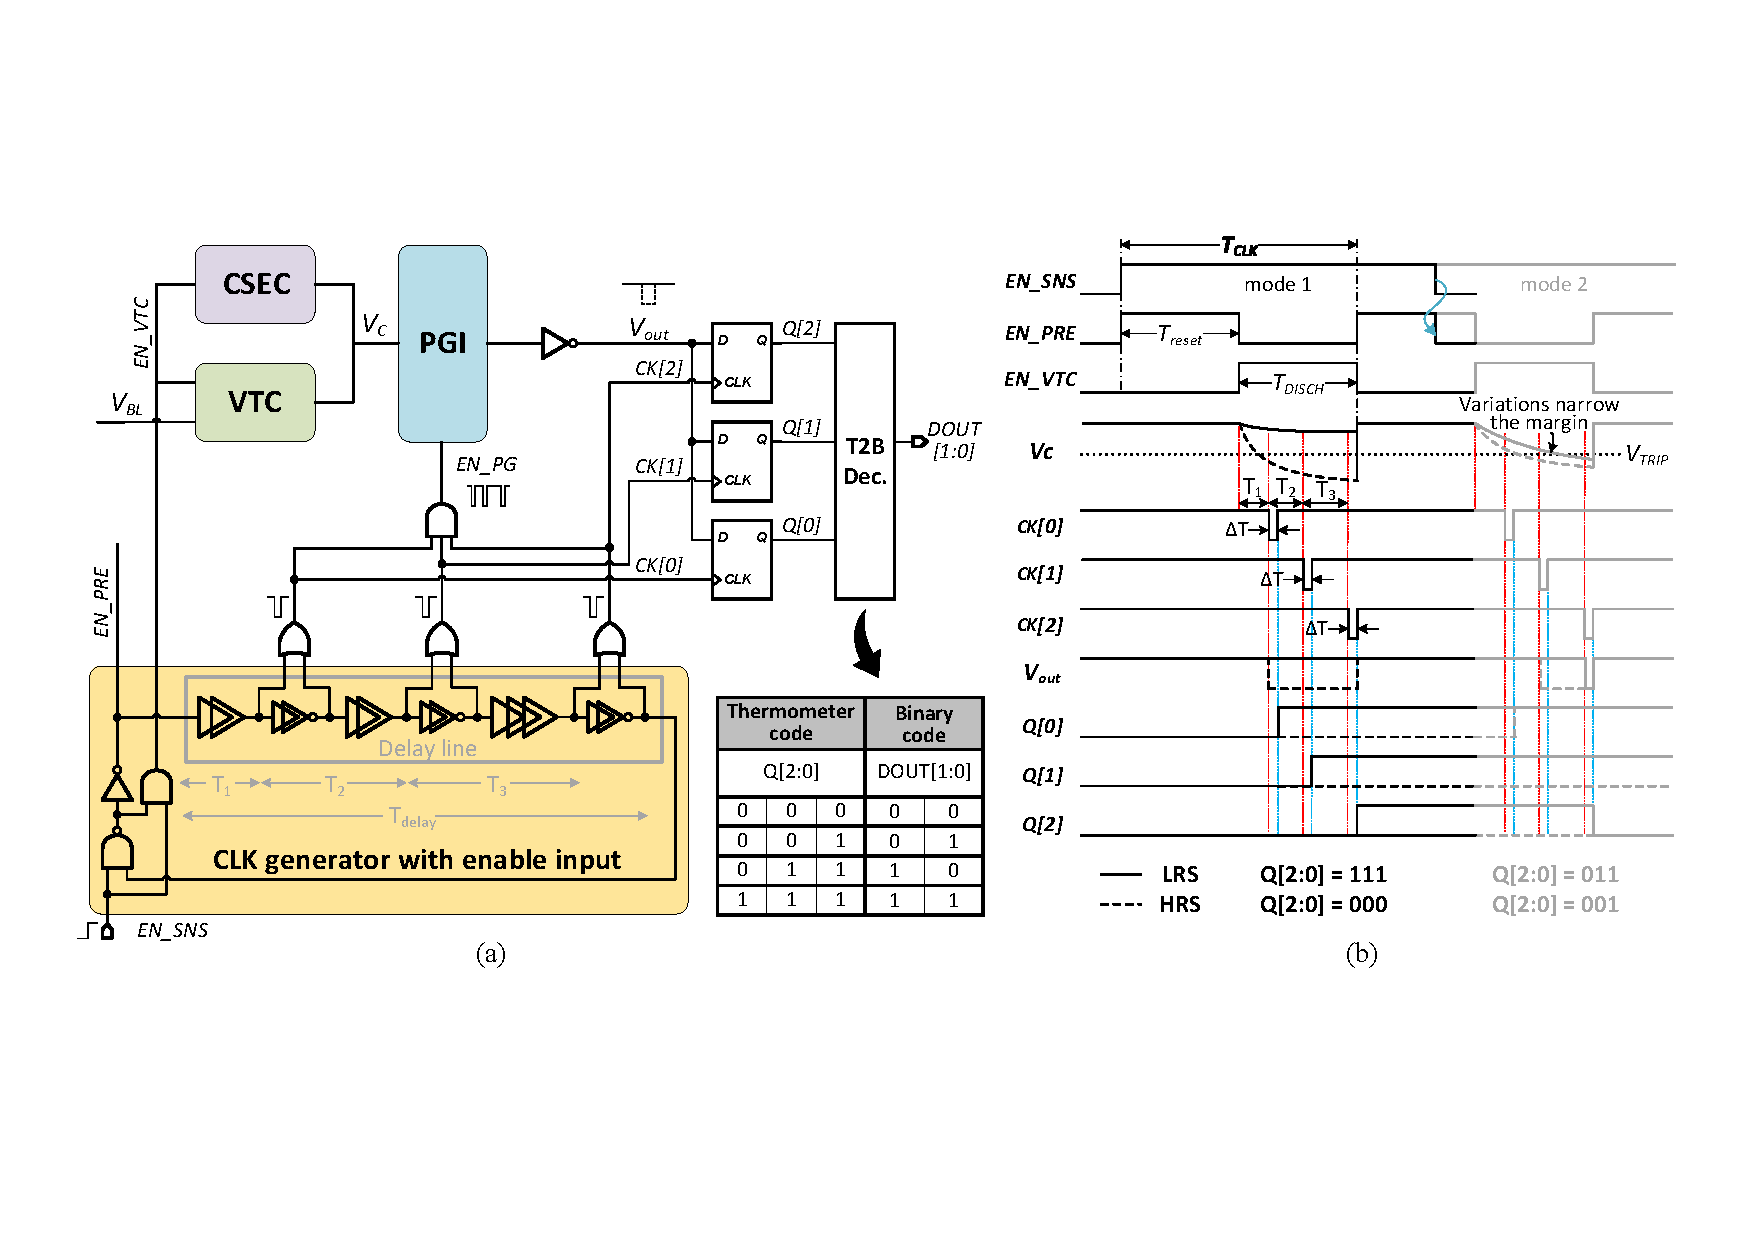
\includegraphics[width=0.98\textwidth]{fig/time_sensing_multiple_new.pdf}}
\caption{Extension of the proposed time-based sensing to multi-level sensing: (a) circuit diagram and the truth table of thermometer code to binary code (T2B) decoder. (b) Typical waveforms of critical nodes for different RRAM states (LRS and HRS) in different readout modes.}
\label{fig_multiple_sensing}
\end{figure*}

The dual-mode timing control block consists of a delay line and a combination logic to generate the control signals for the proposed time-based sense amplifier (TSA). The output of the delay line is fed back to its input as a closed-loop to derive a ring oscillator for automatic reading. The clock generator loop is controlled by the enable signal $EN\_SNS$.

The clock period of the oscillator $T_{CLK}$ depends on the total delay time of the loop. For a stable ring oscillator, the signal must go through each of the delay stages twice to provide one period of oscillation \cite{zhang2021cco}, which can be evaluated by
\begin{align}
\label{eq_clk}
T_{CLK} \approx 2(T_1+\Delta T)
\end{align}
where $T_1$ denotes the delay time of the delay line for RRAM state sensing and voltage developing, and $\Delta T$ denotes the short enable time for PGI to shape the voltage and for the DFF to latch the data, as depicted in Fig. \ref{fig_prop_circuit}(b). 
Although smaller $\Delta T$ consumes lower energy in the PGI, $\Delta T$ should be larger than the propagation delay of the shaping inverters from $V_C$ to $V_{out}$ in order to sample correctly for the DFF.

Fig. \ref{fig_vc} shows 1000 runs MC simulation results of transient $V_{BL}$ and $V_C$ for RRAM in different states, as well as the histogram distribution of $V_C$ at a shorter and longer delay time.
Interestingly, $V_C$ in LRS keeps constant after a short time of discharge because $V_{BL}$ is quickly pulled down to the ground by the low resistance of RRAM. Therefore, the voltage difference of $V_C$ in LRS and HRS increases with the discharge time. 
The discharge time $T_1$ determines the read BER and the read energy, as shown in Fig. \ref{fig_ber_delay}. With a longer delay time, $V_C$ corresponding to HRS goes as low as zero and the voltage window of different states enlarges gradually. As a result, the read operation becomes more reliable and the BER decreases. On the other hand, the sensing energy is almost constant for both HRS and LRS (lower than 50 fJ) over the delay time due to the power gating employed. It is noteworthy that the read energy in HRS consumes $\sim 6$ fJ higher than the read energy in LRS. The extra energy is consumed for resetting $V_C$, considering $V_C$ is discharged much lower in HRS (see Fig. \ref{fig_vc}).
Only negligible static power is consumed during the extended delay time.
% It is important to note, however, extending the delay time too much will increase $BER_{LRS}$, and hence degrade the overall BER.
Theoretically, extending the delay time too much will increase $BER_{LRS}$, and hence degrade the overall BER, as shown in Fig. \ref{fig_BER_probability}. 
In our design, the size of the MOS transistor in the 1T1R bitcell is $W/L$ = 360 nm/40 nm, leading to the maximum discharge current of 100 (85) $\rm \micro$A for bitcell in LRS under a precharge voltage of 400 (300) mV. $V_{BL}$ would be discharged to 100 mV within 2.5 ns, resulting in $V_C$ kept high in LRS and eliminating the limitation of $BER_{LRS}$ in practice. It is important to note that the read access time increases with lower precharge voltage since it takes a longer discharge time to discriminate $V_C$.

The dual-mode timing control logic supports two different readout operation modes according to the pulse width of the enable signal $EN\_SNS$, as listed at the bottom of Fig. \ref{fig_prop_circuit}(a).
\begin{enumerate}
\item[1)] Single Readout Mode\\
When the pulse width of $EN\_SNS$ is set $T_{CLK}<T_{EN\_SNS}<\frac{3}{2}T_{CLK}$, the VTC enable signal $EN\_VTC$ is enabled only once and therefore, the TSA read the state one time, as the black waveforms shown in Fig. \ref{fig_prop_circuit}(b). When $EN\_SNS$ goes low, the TSA is reset for the next sensing.
\item[2)] Multiple Readout Mode\\
If $T_{EN\_SNS} \geq 2T_{CLK}$, the timing control loop activates $EN\_PRE$ and $EN\_VTC$ alternately and the TSA reads the state consecutively, as the grey waveforms shown in Fig. \ref{fig_prop_circuit}(b). With no external controller required, it can read the whole memory array automatically by using the $T_{CLK}$ as the system read clock. Besides, this is also useful in the case of successively reading the same bitcell multiple times for statistical analysis.  
\end{enumerate}



The dual-mode timing controller block includes many buffers in the delay line and correspondingly consumes significant energy (39\%) and areas (43\%). In this work, a $512 \times 512$ 1T1R array is designed, and the timing controller block is shared with all TSAs. Therefore, the overhead distributed into each TSA becomes negligible. 


\section{Extension to Time-based Multi-level Sensing}
\label{sec_features}

As discussed before, the impact of variations and non-linearity of RRAM at the device level degrades sensing reliability and increases the read BER.
By sensing the discharge voltage $V_C$ multiple times, the proposed TSA can be easily extended to multi-level sensing. Fig. \ref{fig_multiple_sensing} illustrates a time-based 3-level sensing scheme, where the logic controller generates 3 enable pulses at different instants of time to PGI for successive sensing. Each of the enable pulse triggers one DFF to store the state, which contributes to the 3-bit thermometer code. Lastly, a thermometer code to binary code (T2B) decoder is used to convert the 3-bit thermometer code to a 2-bit binary code. The truth table of T2B decoder is listed in Fig. \ref{fig_multiple_sensing}(a).

The timing diagrams of critical nodes for RRAM in both LRS and HRS are depicted in Fig. \ref{fig_multiple_sensing}(b) with solid and dash lines respectively. The sensing points are $T_1$, $T_2$ and $T_3$ respectively, with a short enable time of $\Delta T$. In the first cycle, $Q[2:0] = 111 (000)$ for LRS (HRS). To show its robustness, the voltage margin of $V_C$ in the second cycle is narrowed because of variations. The sensing result $Q[2:0] = 011 (001)$ for LRS (HRS), from which we can still discriminate the states. For the single-point sensing, however, it is difficult to sense the state correctly -- if the sensing point is too early (like $CK[0]$), the output is high for both states; if the sensing point is too late (like $CK[2]$), the output is low for both states. This shows the advantage of multi-level sensing with more robust and higher accuracy.

Thanks to the features of time-domain processing, the overhead of the multi-level sensing scheme is only delay stages, compared with the conventional voltage or current mode multi-level sensing schemes. 
Multi-level sensing is beneficial to robust reading and can be applied to multi-level cell (MLC) sensing as well. Next, we will explain these separately.

\begin{figure}[!t]
\centerline
{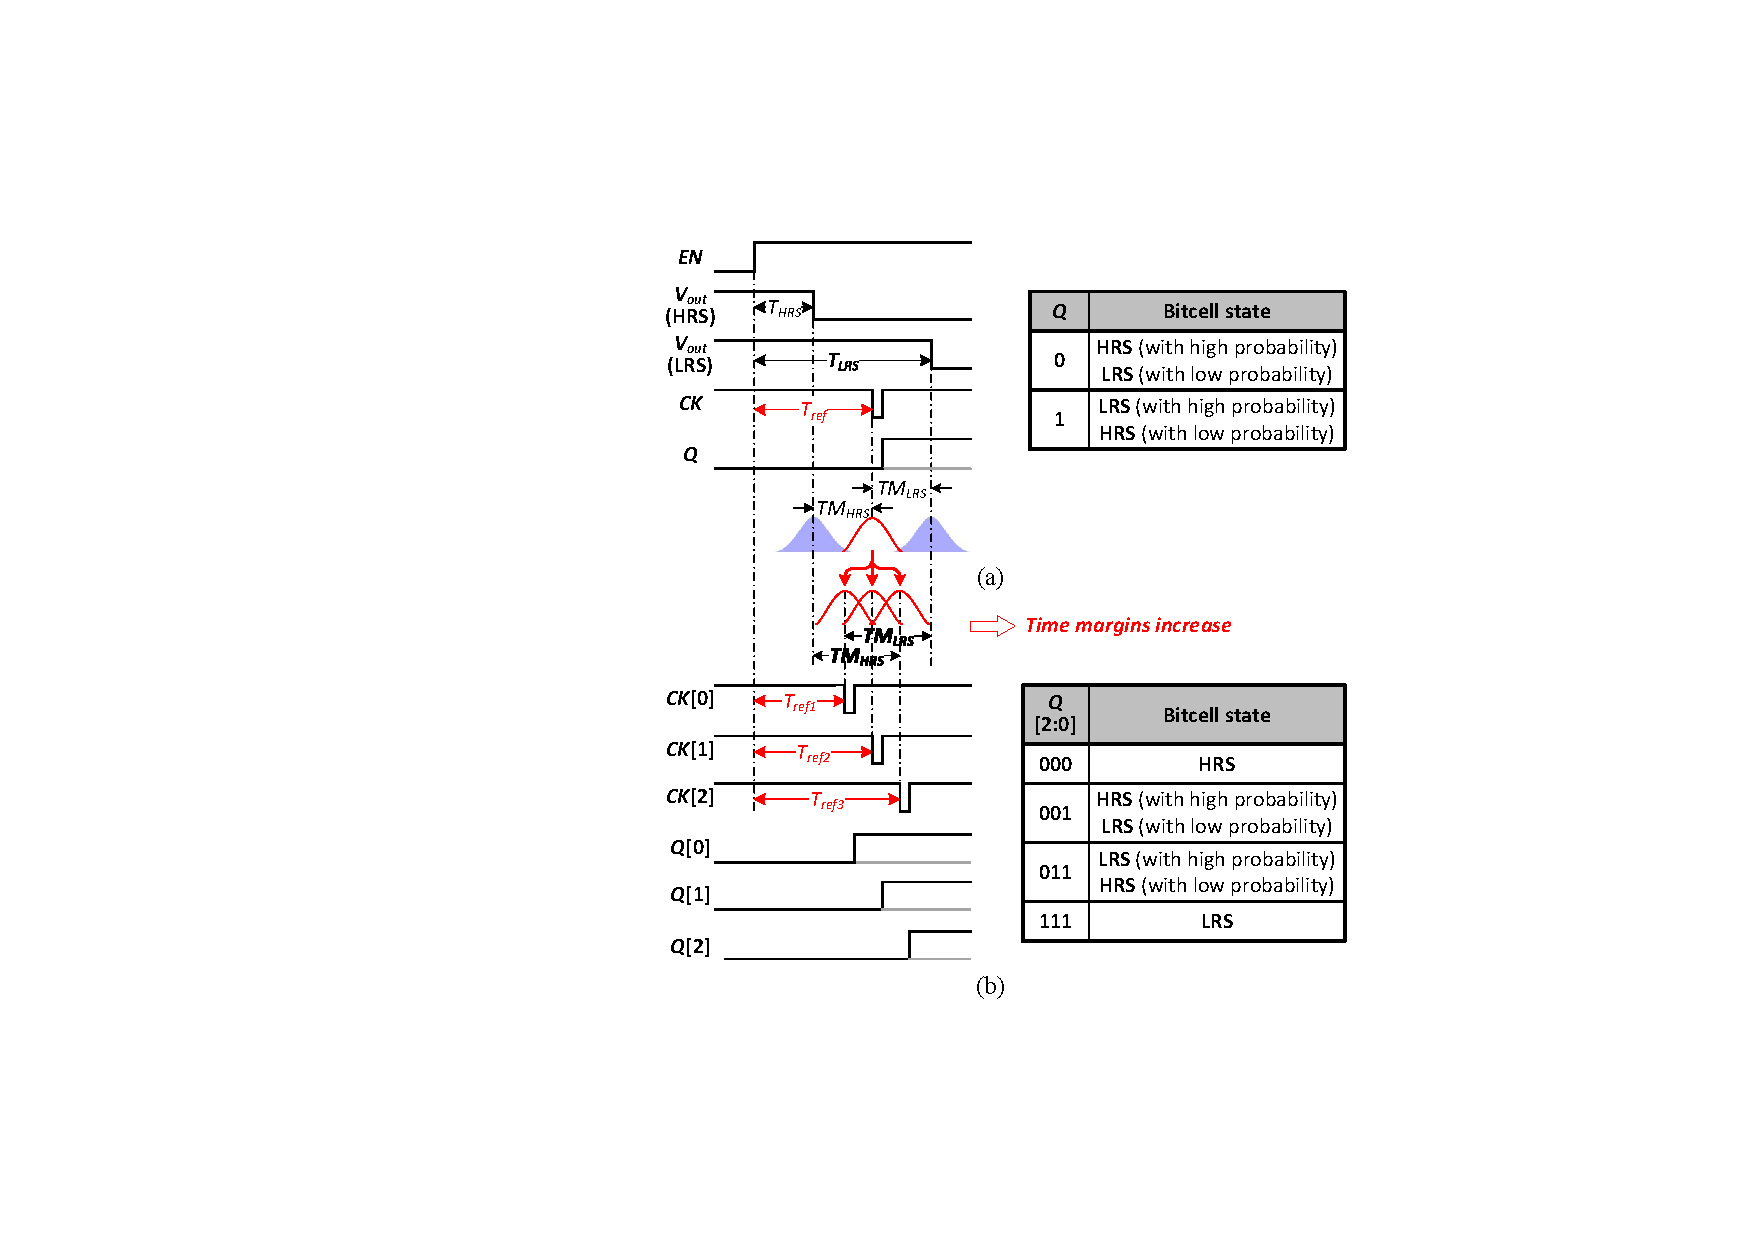
\includegraphics[width=0.46\textwidth]{fig/multi_level_sensing_waveforms_vs_conventional_new.pdf}}
\caption{Timing diagrams and bitcell state for (a) single sensing and (b) multiple sensing. The signal names are the same as Fig. \ref{fig_prop_circuit} and Fig. \ref{fig_multiple_sensing} respectively. Dashed lines represent HRS.}
\label{fig_MLS_compare}
\end{figure}

\subsection{Time-based Multi-level Sensing Technique}
% Conventional time-based sensing detects $V_{out,VTC}$ once and compares it with a reference delay signal $V_{EN,latch}$ to read the bitcell state, as shown in Fig. \ref{fig_sensing_mode}(c). However, the variations of $V_{out,VTC}$ induced by RRAM resistance variation and VTC variation may produce incorrect sensing. 
Conventional sensing schemes detect the state once and compare it with a reference signal to read the bitcell state. However, the fluctuations induced by RRAM resistance variation and sensing circuit variation may produce incorrect sensing. 
Fig. \ref{fig_MLS_compare}(a) shows the typical timing diagrams of a time-based single sensing scheme and the corresponding detection results of the bitcell state. 
To improve sensing accuracy and robustness, a multi-level sensing scheme is proposed, by which multiple points (3 in this case) are sensed consecutively, as shown in Fig. \ref{fig_multiple_sensing}.  
The reference signal is split into three references, assuming $T_{ref}=T_{ref2}$, as shown in Fig. \ref{fig_MLS_compare}(b). The bitcell state is represented by the 3-bit thermometer code $Q[2:0]$. If $Q[2:0]=00\times$, a HRS state is detected; and if $Q[2:0]=\times11$, a LRS state is detected. That is to say, the criteria for HRS are $T_{ref2}$ and $T_{ref3}$ -- the overall reference time $T_{ref,H}$ for HRS is longer than $T_{ref}$; the criteria for LRS are $T_{ref1}$ and $T_{ref2}$ -- the overall reference time $T_{ref,L}$ for LRS is shorter than $T_{ref}$. The time-based multi-level sensing scheme is actually converter the single reference in single sensing scheme to dynamic references -- shorter (longer) time reference for LRS (HRS) detecting. Therefore, both the time margins $TM_{LRS}$ and $TM_{HRS}$ increase. 

As discussed in section \ref{challenges}, $BER_{HRS}$ declines with longer reference time $T_{ref}$ and $BER_{LRS}$ declines with shorter reference time $T_{ref}$ (see  Fig. \ref{fig_BER_probability}). 
Compared to the single sensing scheme, both $BER_{HRS}$ and $BER_{LRS}$ are declined in the multi-level sensing scheme, resulting in a lower overall BER. This makes the multi-level sensing scheme more robust and accurate. 


\subsection{Application to Multi-level Cell (MLC) Sensing}

\begin{figure}[!t]
\centerline
{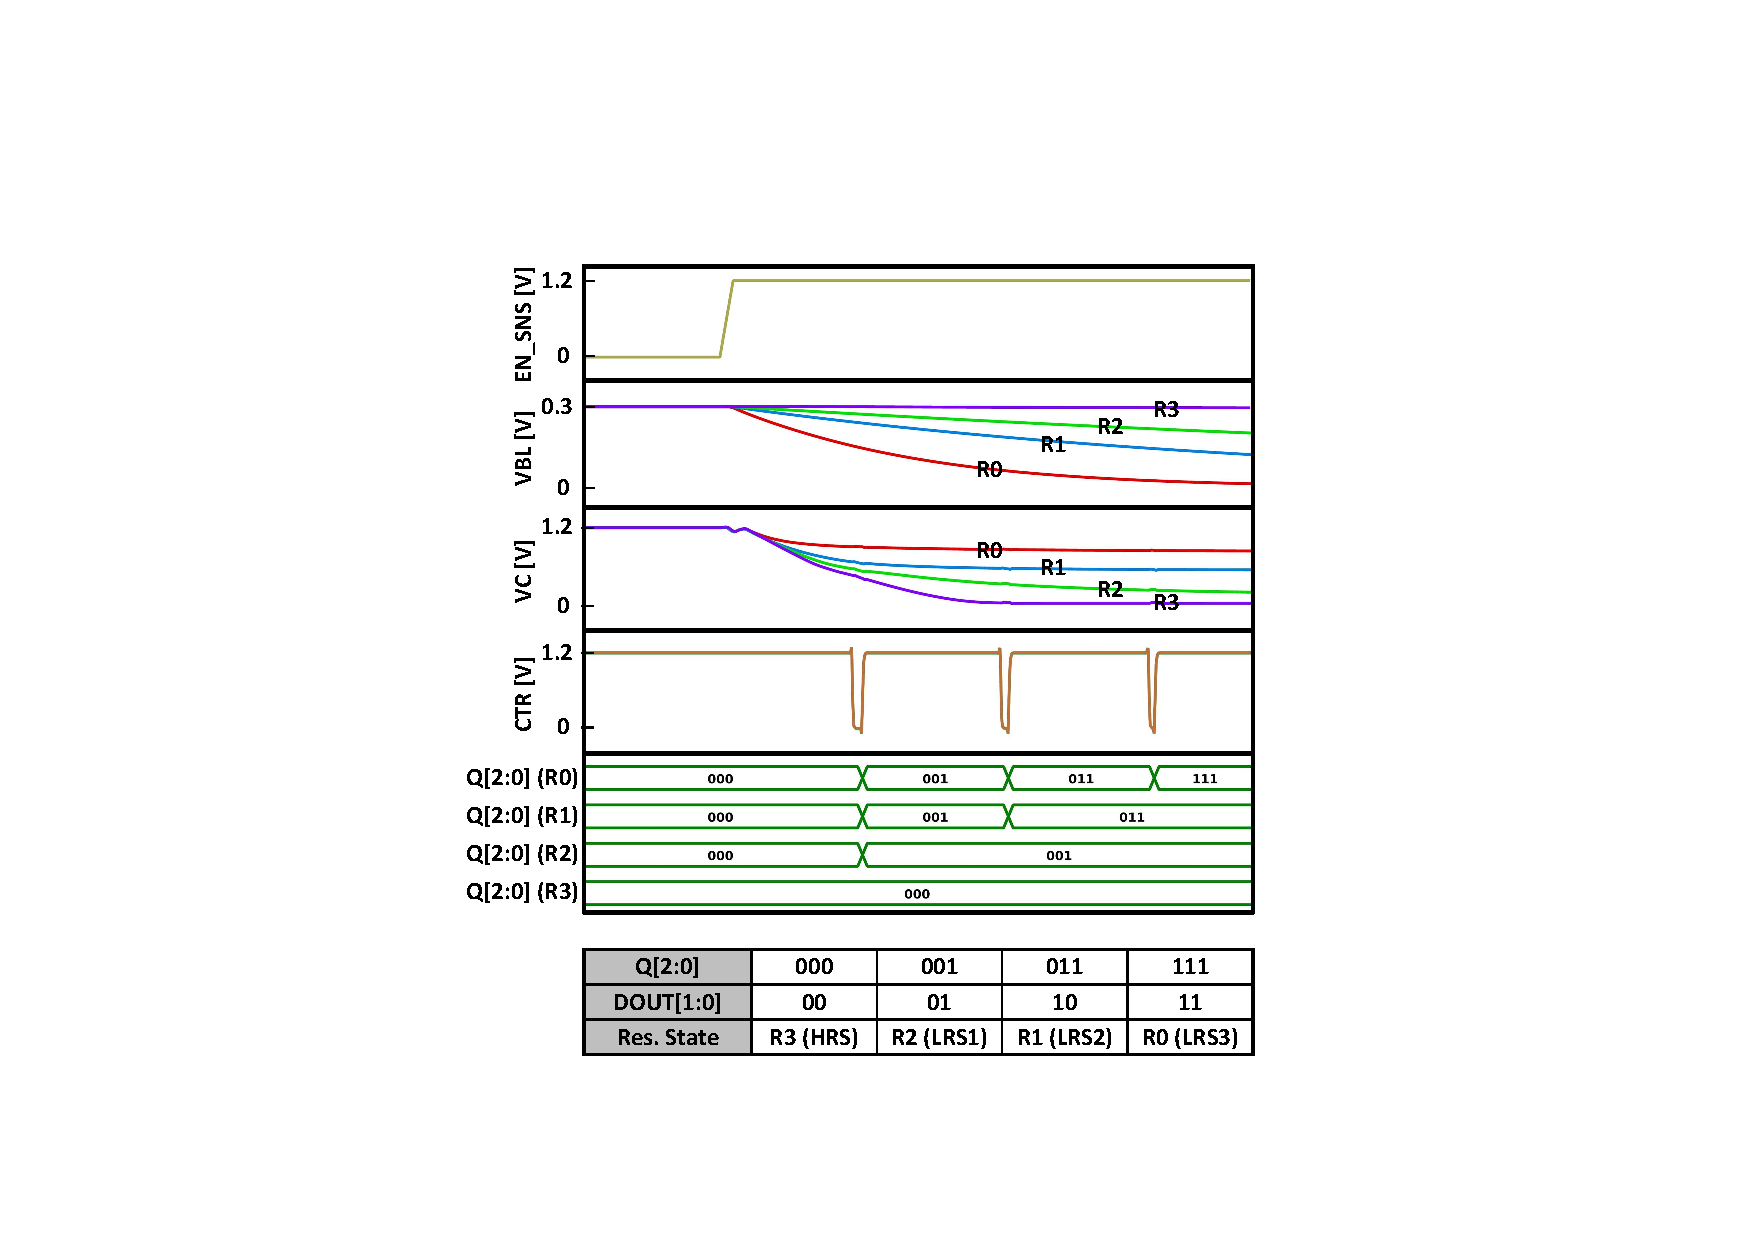
\includegraphics[width=0.49\textwidth]{fig/multi-level_sensing.pdf}}
\caption{Timing diagrams and bitcell states for 2-bit MLC RRAM sensing. The resistance decreases with the number of bit "1" detected in the output $Q[2:0]$.}
\label{fig_multi_level_sensing}
\end{figure}

The demand for increasing memory density has motivated researchers to store more bits per cell by implementing Multi-Level Cell (MLC) or multi-bit RRAM \cite{reuben2019time}.
MLC would be implemented by modulating (1) the compliant current, (2) programming voltage amplitude, or (3) programming pulse width \cite{prakash2016multilevel}.


% To simulate the BER for both HRS and LRS, the delay loop in Fig. \ref{fig_multiple_sensing} is broken to discharge $V_C$ freely. 
The proposed time-based multi-level sensing scheme also supports the detection of MLC RRAM. As an example, a 3-level consecutive sensing scheme can detect four different RRAM states (2-bit). Fig. \ref{fig_multi_level_sensing} depicts the sensing waveforms, the digital results, and the corresponding resistance states. 
Different resistance states develop different $V_{BL}$ levels (in this case, $R3>R2>R1>R0$), resulting in different discharge speeds of $V_C$. 
The state of MLC RRAM is detected by comparing voltage $V_C$ with trip voltage $V_{TRIP}$ of the subsequent inverter at three different times and decoding the latch results. The sensing results and the resistance states are listed at the bottom of Fig. \ref{fig_multi_level_sensing}.
In general, to sense $N$-bit MLC RRAM, the time-based sensing needs consecutively sense the state at $2^N-1$ time points. 


\section{Simulation Evaluation of Time-based Sensing and Comparison with Other Sensing Schemes}
\label{sec_results}
\subsection{Read Access Time and Energy}

\begin{figure}[!t]
\centerline
{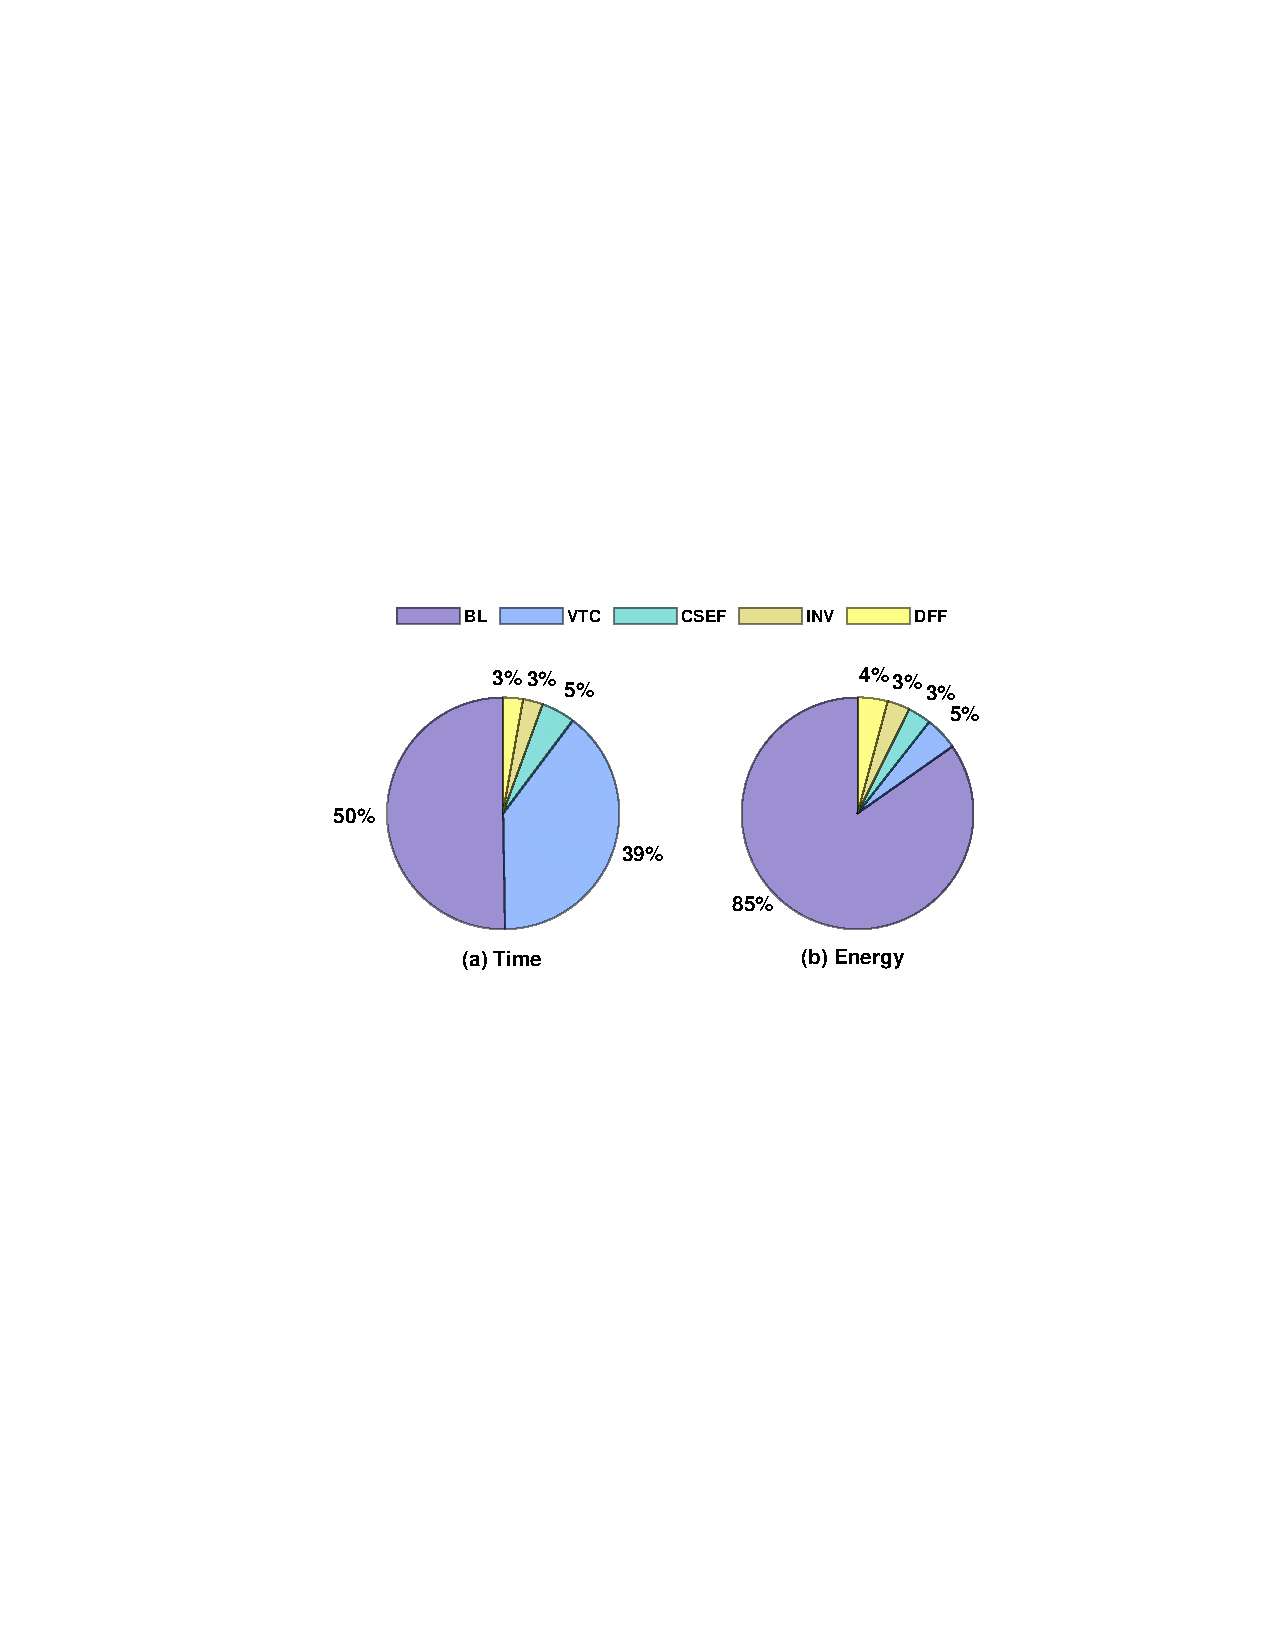
\includegraphics[width=0.46\textwidth]{fig/time_energy_pie_new.pdf}}
\caption{Breakdown of (a) read access time and (b) energy under supply voltage of 1.2 V.}
\label{fig_time_energy_pie}
\end{figure}

To evaluate the overall performance of the proposed TSA, we designed a typical sub-bank size of $512\times512$ 1T1R bitcells with 16:1 column multiplexing for the readout circuit, where each TSA is shared by 16 columns. The simulations are performed under the adopted 40-nm technology, as mentioned in Section \ref{sim_model}. 

In each read cycle, the overall read access time $T_{read}$ is divided into the time of $T_{reset}$ to precharge the bitline voltage $V_{BL}$ and the time of $T_{DISCH}$ associated with the VTC and state detection. 
%$T_{read}$ is set by the time $T_{PRE}$ to charge the bitline voltage $V_{BL}$ to precharge voltage $V_{PRE}$, and the sensing delay $T_{sense}$ associated with the sense amplifier.  
$T_{DISCH}$ is equal to the summation of the time of the delay line $T_1$ ($T_1 + T_2 + T_3$) for single-level (multi-level) sensing schemes and the PGI enable time $\Delta T$, as shown in Fig. \ref{fig_prop_circuit} (Fig. \ref{fig_multiple_sensing}). 
In this work, $T_{reset}$ and $T_{DISCH}$ are equal since they represent the positive half and negative half of the clock signal generated by the timing control loop. 
% The clock period is designed as 10 ns to set the read frequency to 100 MHz. So the sensing time ($T_{DISCH}$) is 5 ns, which is enough to develop bitline voltage and discriminate $V_C$ accurately according to Fig. \ref{fig_ber_delay}. 
The size of the precharge NMOS transistor is determined by the bitline parasitic capacitors $C_{BL}$ and precharge voltage $V_{PRE}$ under the given precharge time.
% It is to be noted that the precharge time $T_{PRE}$ depends on the bitline parasitic capacitors $C_{BL}$ and the size of the precharge NMOS transistor.
The breakdown of the read access time is shown in Fig. \ref{fig_time_energy_pie}(a). The bitline precharge time takes 50\% of the read access time, and another 39\% is taken by the transition of $V_C$ after the VTC is enabled. Bitline precharge and VTC transition account for the major proportion of the total time. The CSEF occupies 5\% of the time to avoid the charge sharing-induced error and expand the read margin efficiently. The shaping inverters and the DFF latch take 3\% of the time equally. 

The read access energy consumed by the proposed TSA comprises four components that can be expressed as 
\begin{align}
\label{eq_energy}
E_{read} \approx E_{BL}+E_{VTC}+E_{CSEF}+E_{INV}+E_{DFF}
\end{align}
where $E_{BL}$ is the energy to precharge the bitline, $E_{VTC}$ is the energy consumed by the VTC, $E_{CSEF}$ is the energy drawn by the CSEF. $E_{INV}$ is the energy drawn by the PGI and the subsequent inverter to shape the signal. $E_{DFF}$ is the energy consumed by the DFF latch. The energy taken by the delay line is neglected in Eq. \eqref{eq_energy}, considering the fact that the delay line is shared by all the bitlines being read simultaneously.
As shown in Fig. \ref{fig_ber_delay}, the read access energy per bit is 49 fJ and 43 fJ under supply voltage of 1.2 V for HRS and LRS respectively. The total energy consumption breakdown is illustrated in Fig. \ref{fig_time_energy_pie}(b). Precharging the bitline consumes the vast majority, to be specific, 85\% of the total energy. The rest are almost equally contributed by the VTC, CSEF, INV and DFF, respectively. 
The energy-efficient shaping inverters benefit from the power gating technique.

% \begin{figure}[!t]
% \centerline
% {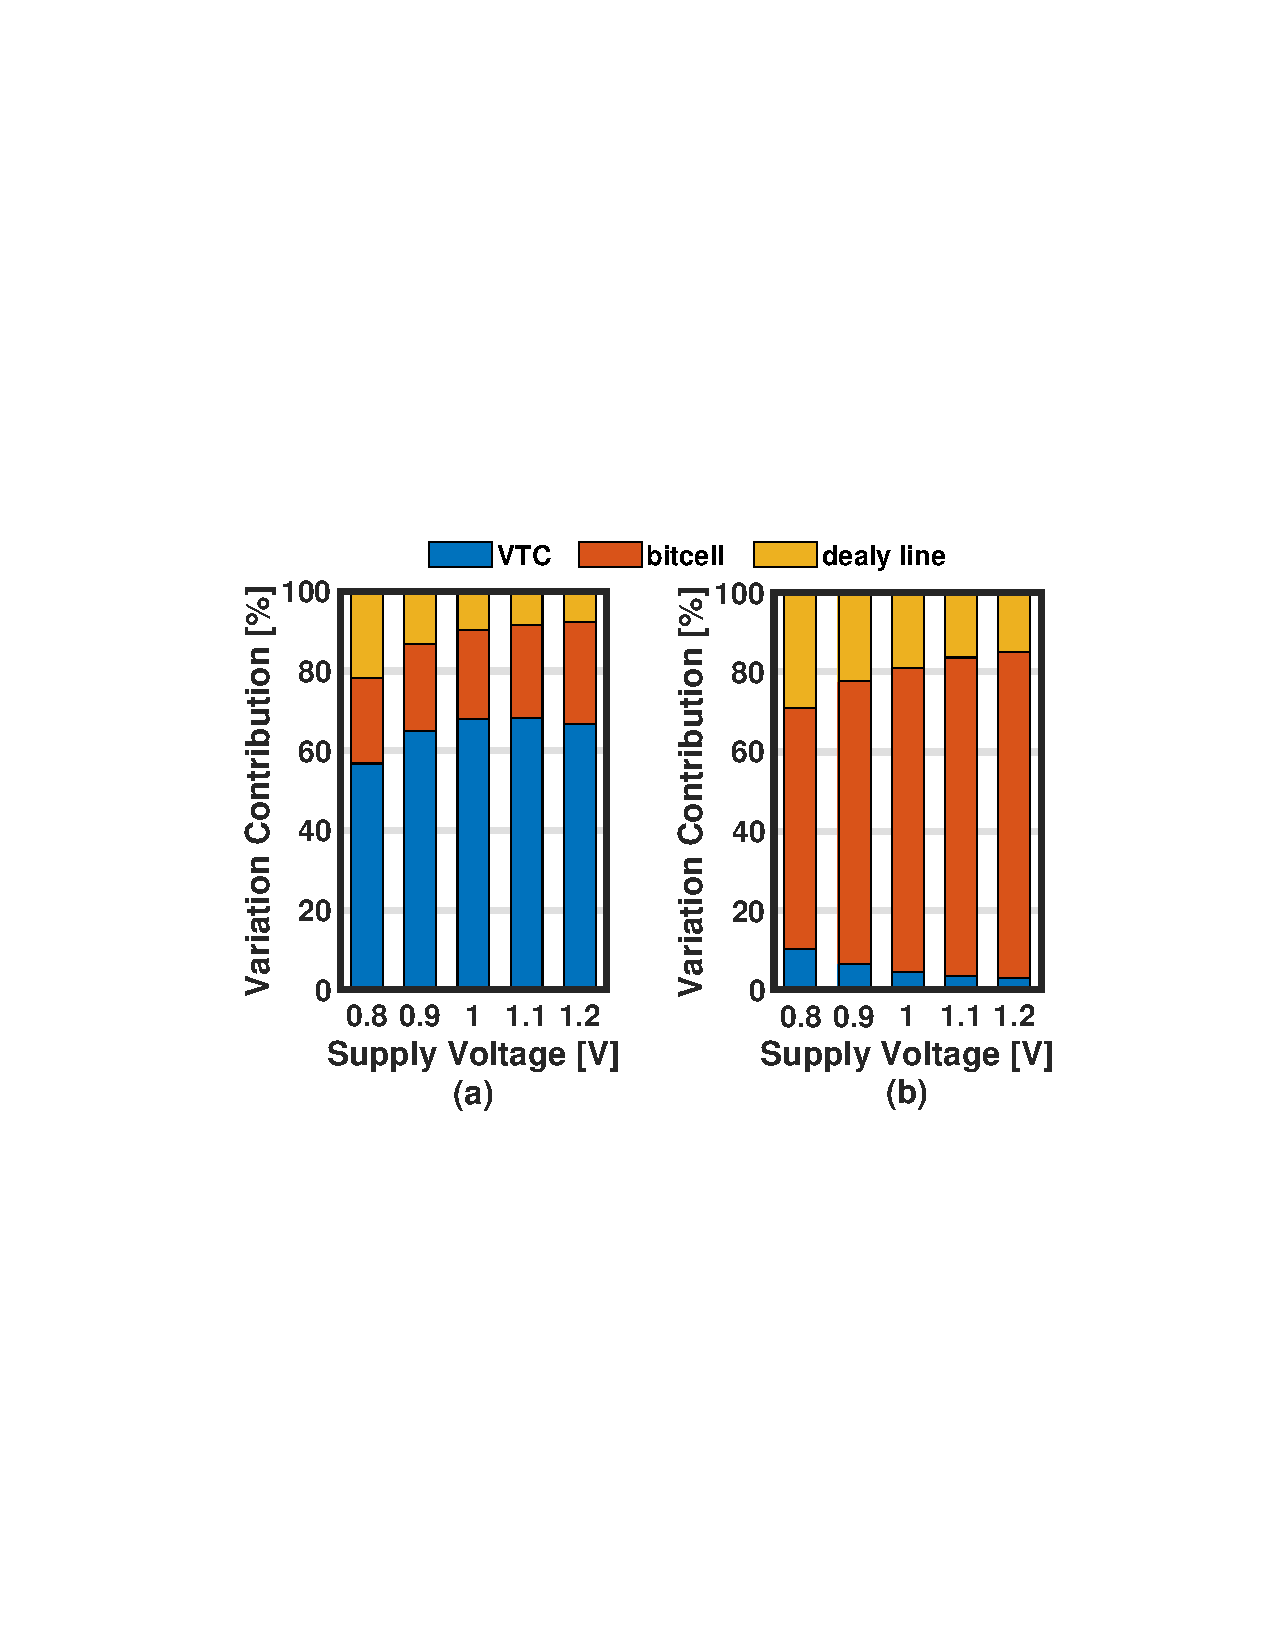
\includegraphics[width=0.45\textwidth]{fig/variation_with_vdd.pdf}}
% \caption{Variation contribution of the TSA when RRAM is in (a) HRS and (b) LRS with different supply voltage.}
% \label{fig_variation_with_vdd}
% \end{figure}

% \begin{figure}[!t]
% \centerline
% {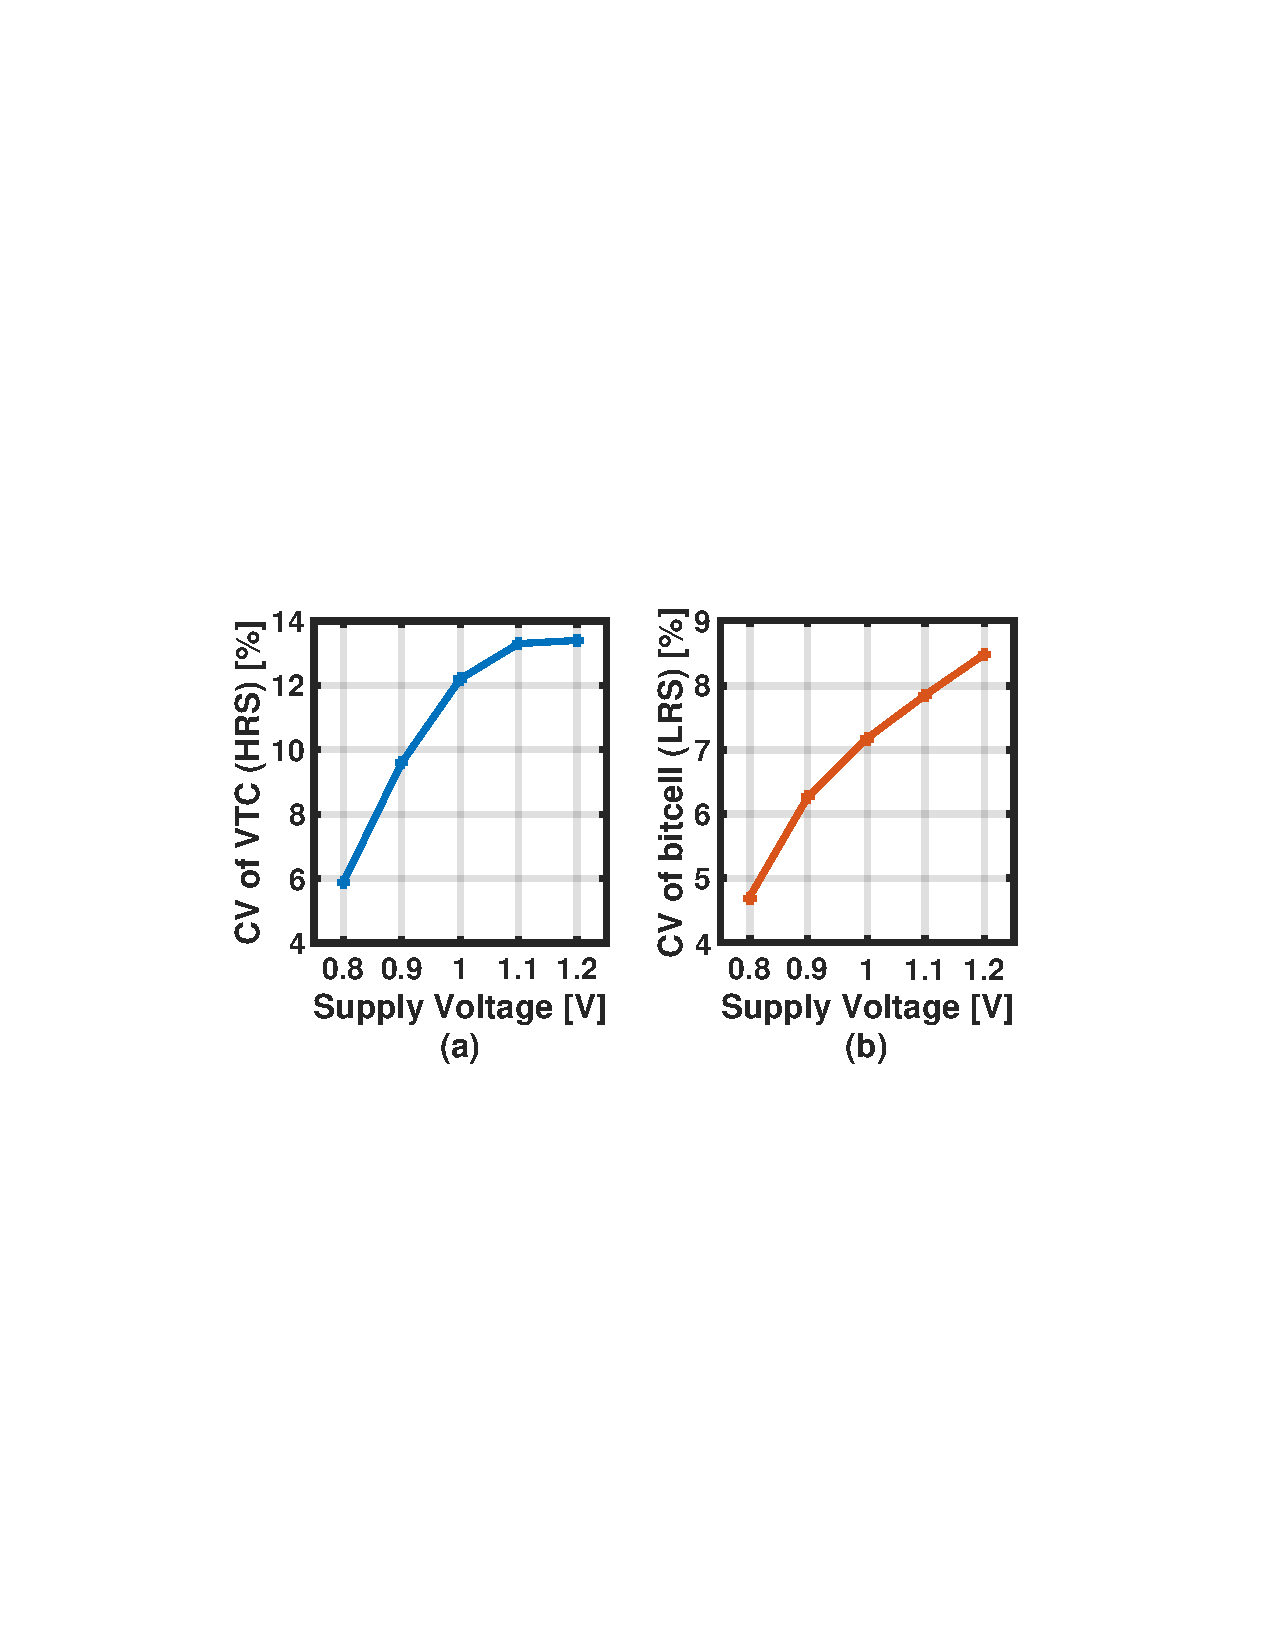
\includegraphics[width=0.45\textwidth]{fig/variation_with_vdd_absolute.pdf}}
% \caption{The coefficient of variation of (a) VTC when RRAM is in HRS and (b) bitcell when RRAM is in LRS with respect to supply voltage.}
% \label{fig_variation_with_vdd_abs}
% \end{figure}

\begin{figure}[!t]
     \centering
     \begin{subfigure}[(b)]{0.44\textwidth}
         \centering
         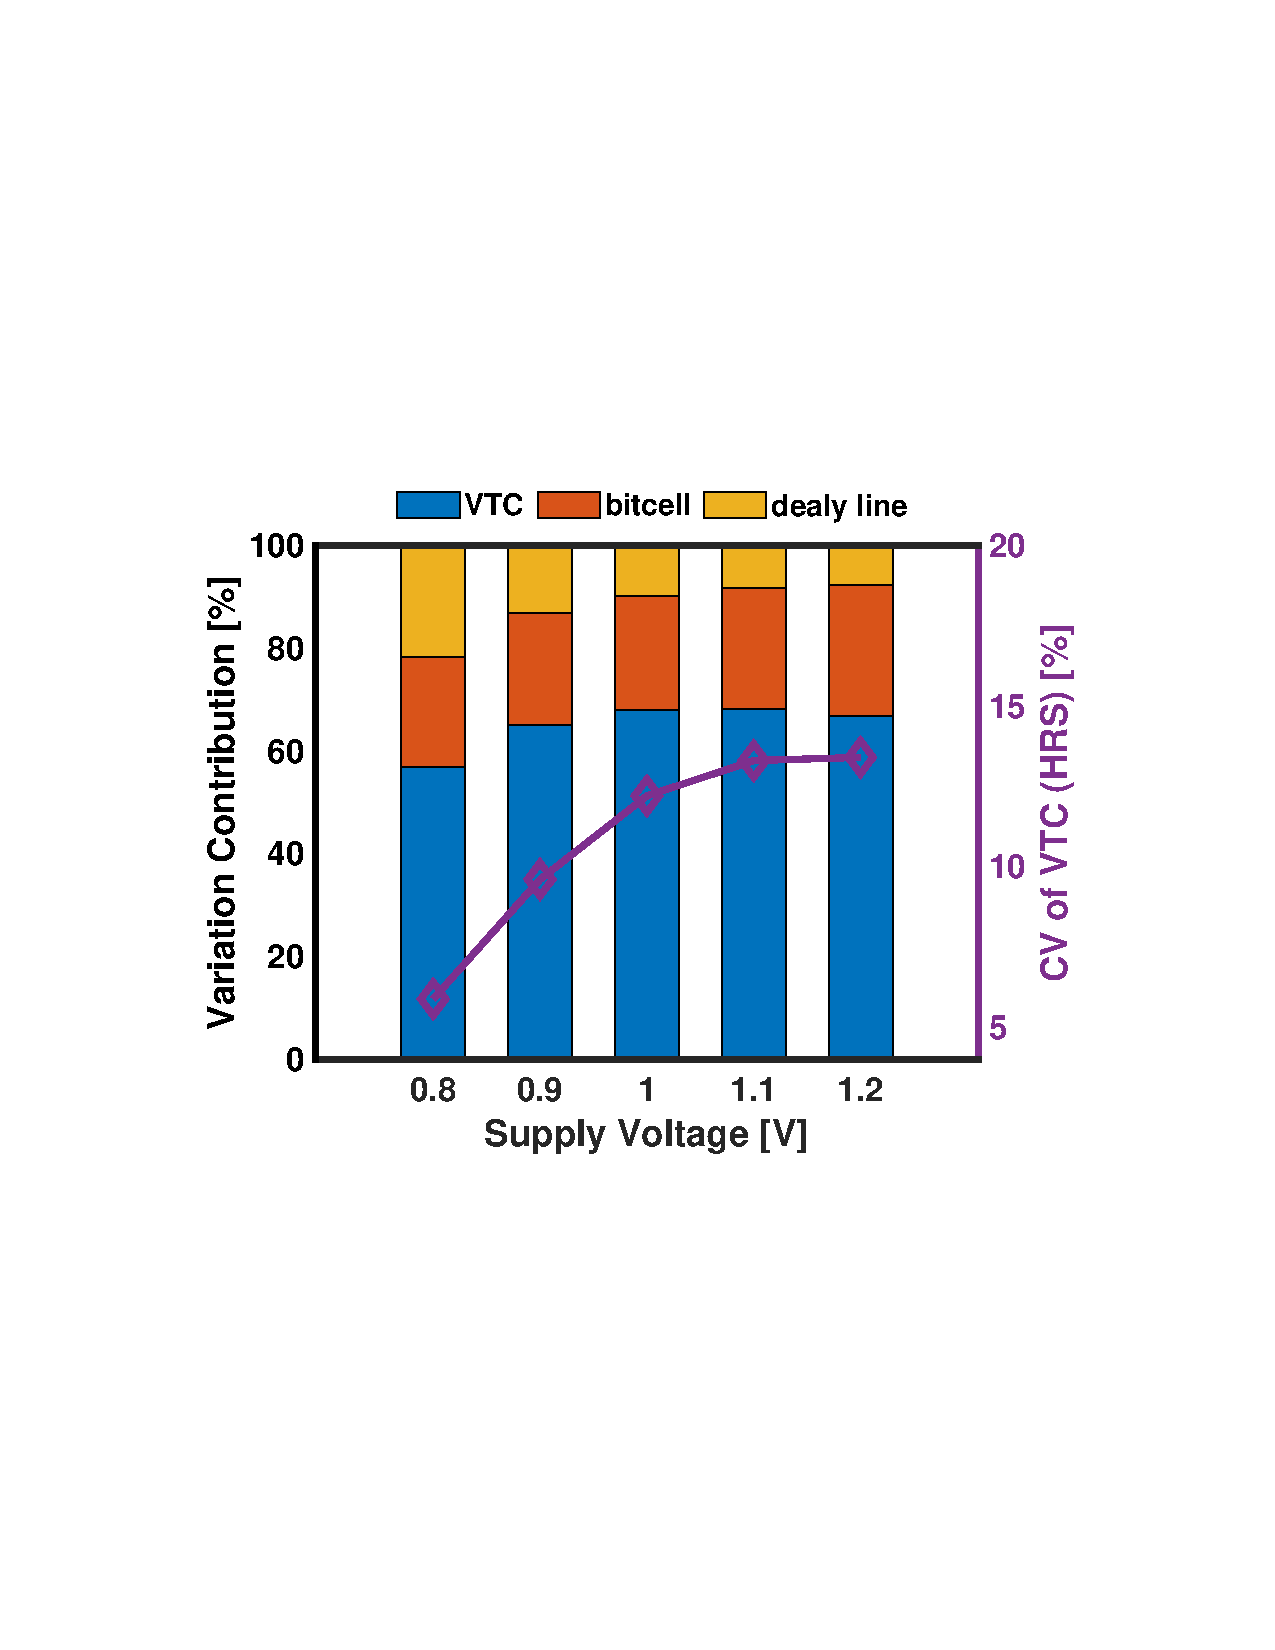
\includegraphics[width=0.9\textwidth]{fig/variation_hrs.pdf}
         \caption{}
         \label{fig_variation_hrs}
     \end{subfigure}
     \par\smallskip 
     \begin{subfigure}[b]{0.44\textwidth}
         \centering
         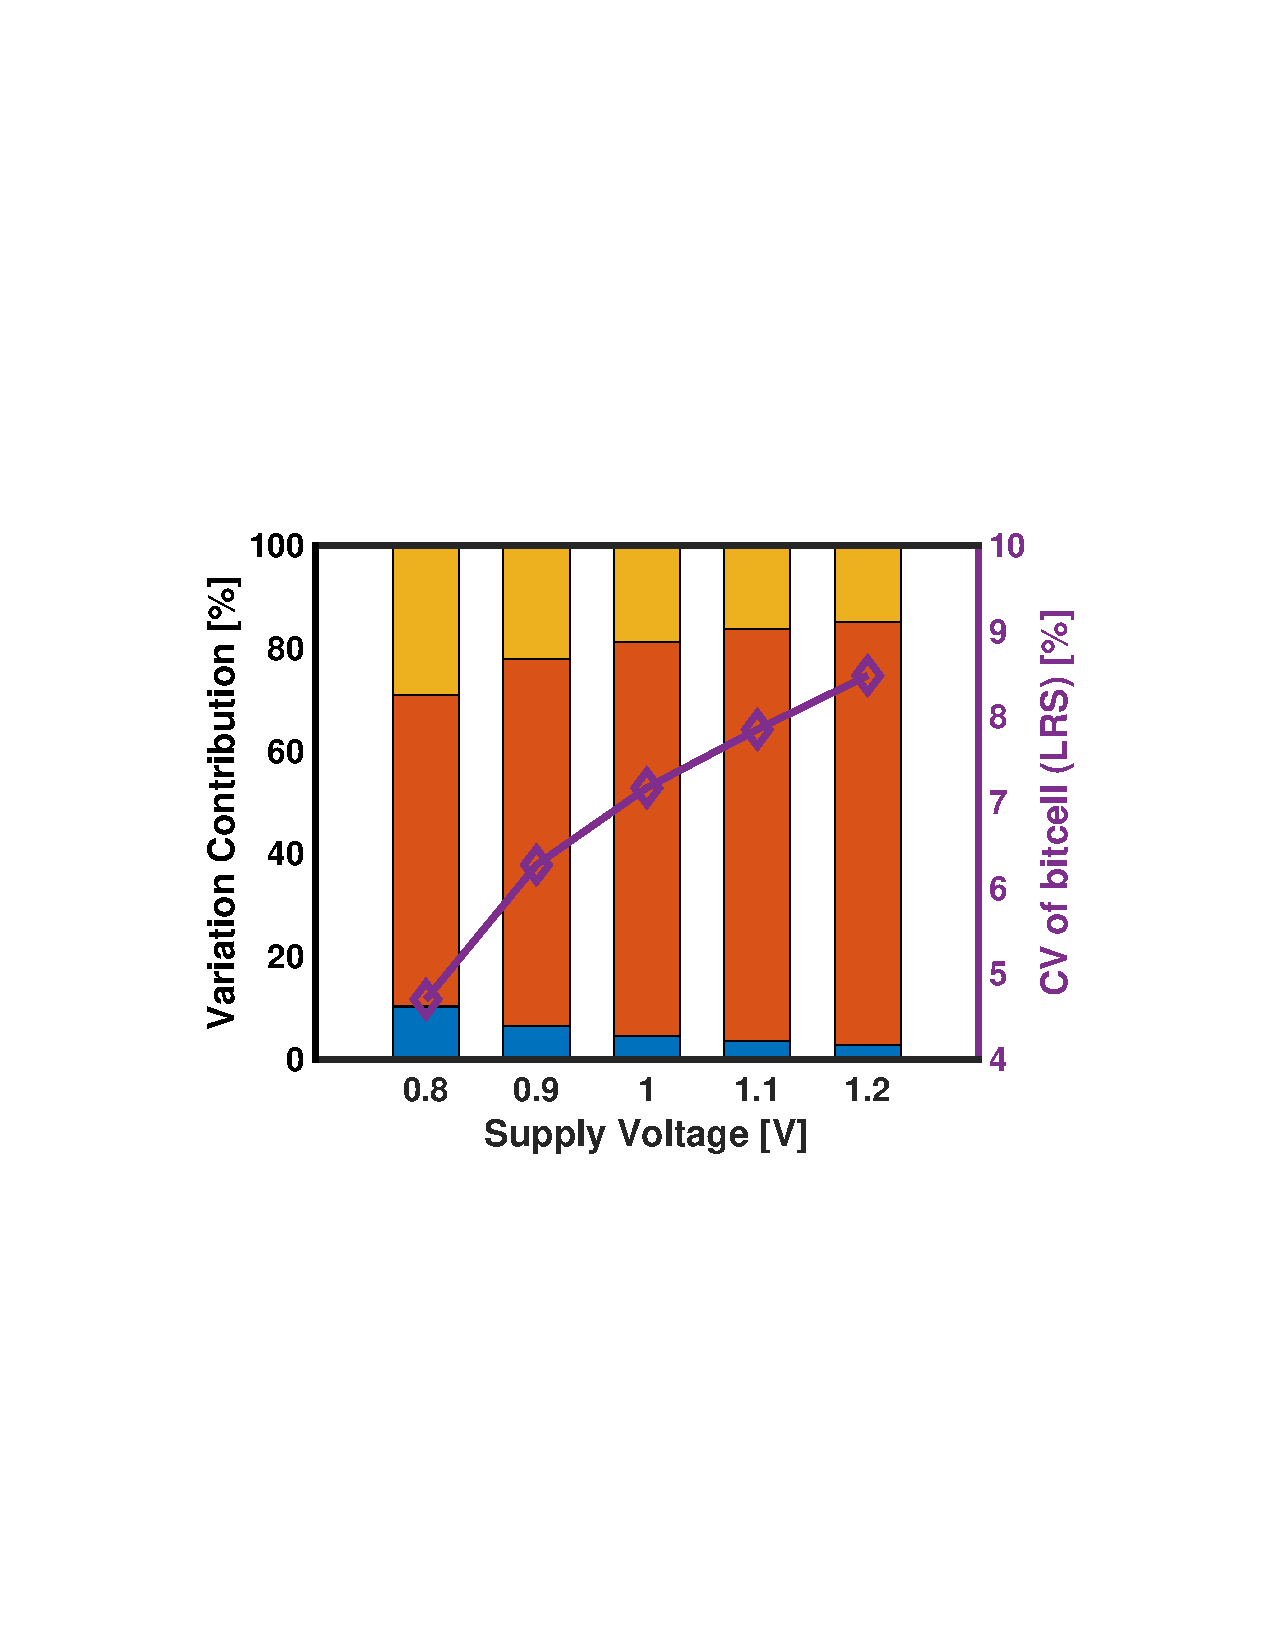
\includegraphics[width=0.9\textwidth]{fig/variation_lrs.pdf}
         \caption{}
         \label{fig_variation_lrs}
     \end{subfigure}
     
     \caption{Variation contribution of the TSA and the coefficient of variation (CV) of the major factor under different supply voltages when the RRAM is in (a) HRS and (b) LRS. The major contributors are VTC and bitcell respectively.}
     \label{fig_variation_with_vdd}
\end{figure}


\subsection{Robustness and Trade-offs}

To study the individual contributors to the overall variations, MC simulations are performed by enabling each block of the proposed TSA respectively. Fig. \ref{fig_variation_with_vdd} reports the variations contributed by the three main sources (i.e., VTC, the bitcell, and the delay line) versus the supply voltage. 
When the RRAM is in HRS, the VTC block is the dominant contributor to the variation, accounting for approximately $60 \sim 70\%$ under different supply voltage, as shown in Fig. \ref{fig_variation_hrs}. That is because the pull-down current, in this case, is relatively large and the output $V_C$ is charged from $V_{DD}$ to a lower voltage close to zero with variations. The bitline voltage almost keeps at the precharge voltage because of the high resistance of RRAM, resulting in a small variation ($\approx 20\%$). To evaluate the absolute variation of the major factor, the coefficient of variation (CV, which is defined as $\sigma/\mu \times 100$) of VTC when RRAM is in HRS is plotted in Fig. \ref{fig_variation_hrs} as well. The VTC variation increases with supply voltage and tends to be saturated when the supply voltage is higher than 1.1V.

When the RRAM is in LRS, the bitline will be discharged by the bitcell current, which is determined by both the low resistance of the RRAM device and the NMOS transistor, making the bitcell variation the dominant contribution ($\approx 60 \sim 80\%$), as shown in Fig. \ref{fig_variation_lrs}. In contrast, the variation of VTC is minimal ($\leq 10\%$) because $V_C$ almost keeps constant in this case. The CV of bitcell when the RRAM is in LRS is plotted in Fig. \ref{fig_variation_lrs} as well. The bitcell variation also increases with supply voltage, but overall, the variation contributed by bitcell when the RRAM is in LRS is lower than that by VTC when the RRAM is in HRS.
% The dominant contributions for the variation in HRS and LRS are the VTC and bitcell, respectively.


\begin{figure}[!t]
\centerline
{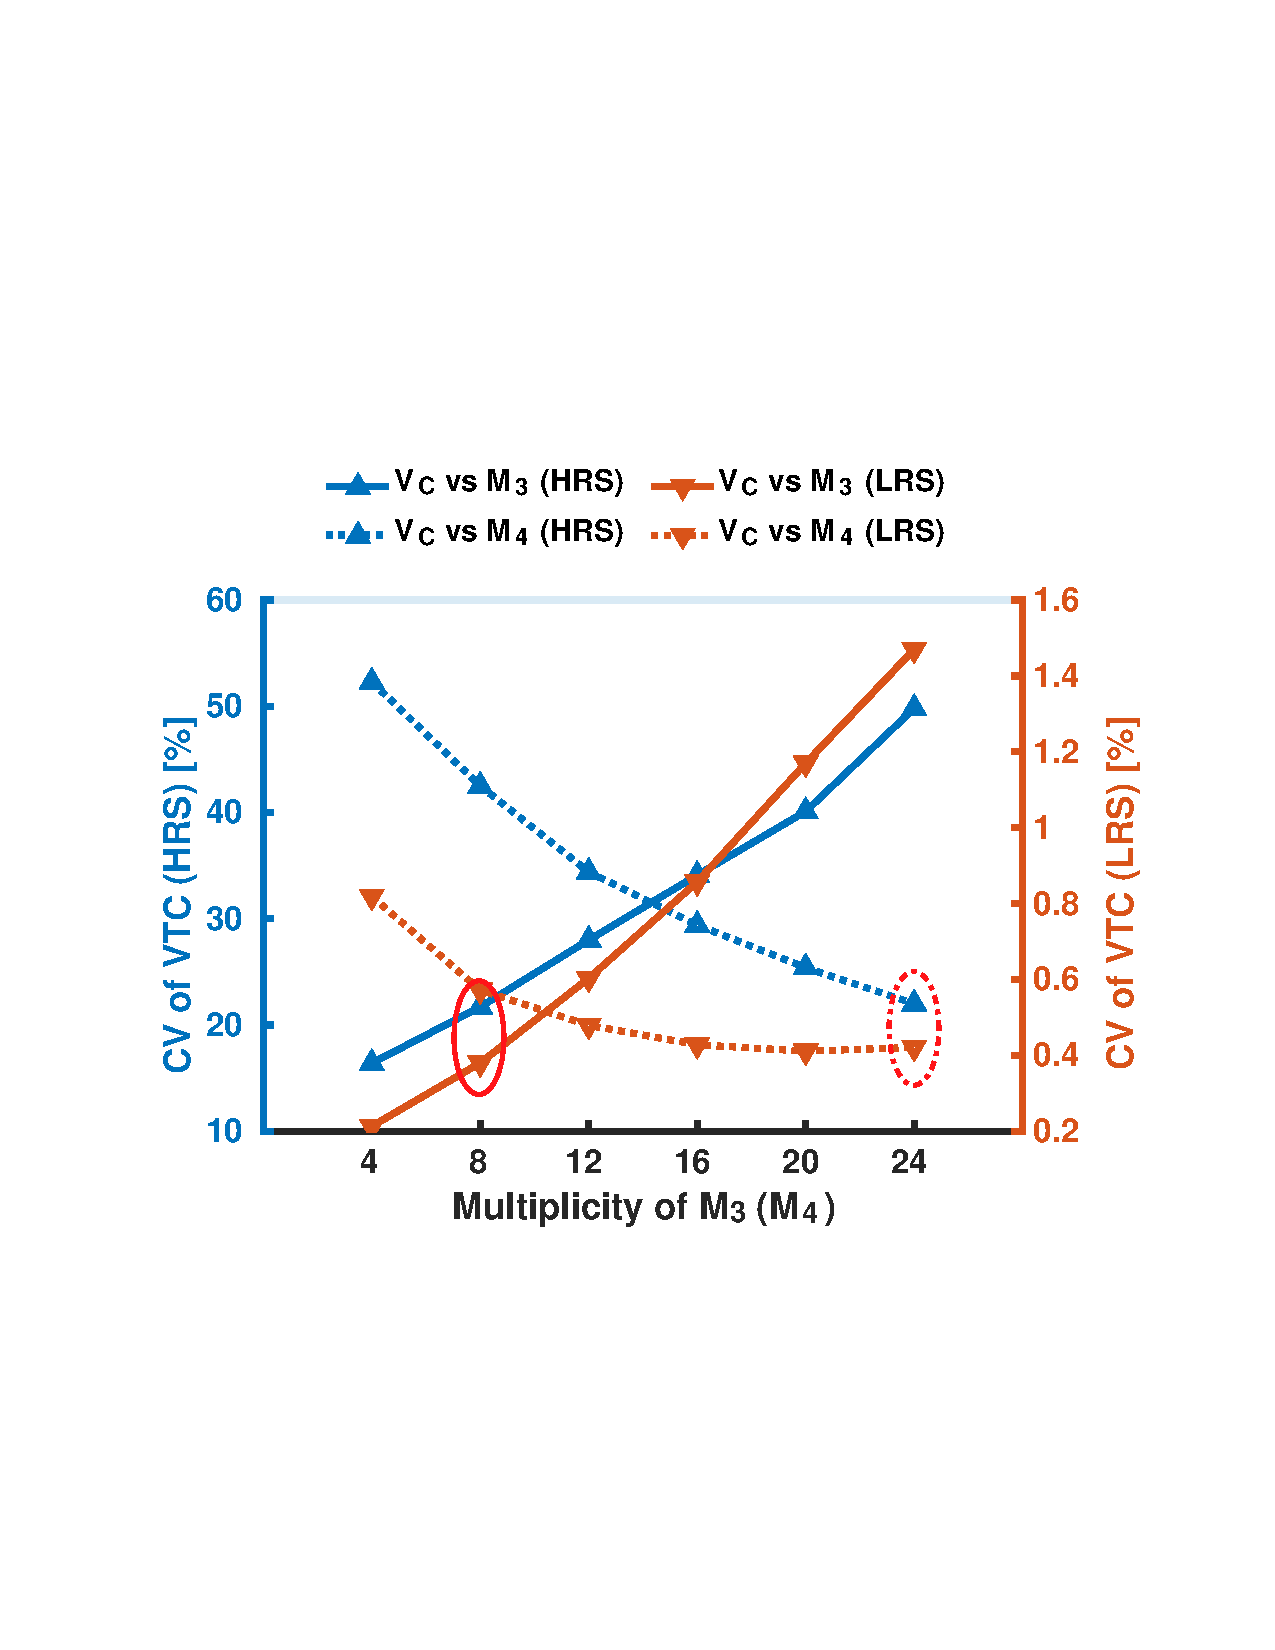
\includegraphics[width=0.44\textwidth]{fig/cv_of_vtc.pdf}}
\caption{The coefficient of variation (CV) of the VTC versus the multiplicity of $M_3$ (the $M_4$ multiplicity is set to 24) and $M_4$ (the $M_3$ multiplicity is set to 8).}
\label{fig_cv_vtc}
\end{figure}

\begin{table*}[ht!]%[htbp]
\centering
\caption{Comparison of the proposed TSA with Conventional VSA and CSA}
\label{tab_performance_comp}
\begin{threeparttable}
\begingroup
\setlength{\tabcolsep}{3pt} % Default value: 6pt
\renewcommand{\arraystretch}{1.5} % Default value: 1
\begin{tabular}{@{}m{3cm}<{\centering}m{2cm}<{\centering}m{4cm}<{\centering}m{2cm}<{\centering}m{2cm}<{\centering}m{2cm}<{\centering}@{}}
\toprule[1.5pt]
Types of SA & Structure & Reference used & BER & Read energy & Read time\tnote{*}  \\ \hline
\midrule
Conventional VSA & Latch-based & $V_{ref}=\frac{1}{2}(V_{BL,L}+V_{BL,H})$ & 6.2E-7 & 45 fJ & 6 ns\\\hline
Conventional CSA & Latch-based & $I_{ref}=\frac{1}{2}(I_{BL,L}+I_{BL,H})$ & 1.5E-6 & 96 fJ & 6 ns\\\hline
Proposed TSA & VTC-based & internal delay & 1E-10 & 49 fJ & 6 ns\\
\bottomrule[1.5pt]
\end{tabular}
% \textcolor{red}{
\begin{tablenotes}
\item[*] The precharge time and developing time are set to be same for a fair comparison of BER.
% \item[**] BER is $4\times10^{-6}$ when read time is 5 ns.
\end{tablenotes}
% }
\endgroup
\end{threeparttable}
\end{table*} 



The variation of the VTC in HRS is dominated by the variations of NMOS transistor $M_3$ and $M_4$, which determine the VTC current and the gate capacitance, respectively.
To gain an insight into the inter-dependence of robustness, performance, and energy for the RRAM sensing circuit, Fig. \ref{fig_cv_vtc} depicts the coefficient of variation of the VTC versus the multiplicity of $M_3$ (the $M_4$ multiplicity is set to 24) and $M_4$ (the $M_3$ multiplicity is set to 8). As discussed before, the CV of the VTC when RRAM is in LRS is much smaller than that when RRAM is in HRS. 
Interestingly, the trends of the curves are similar in both HRS and LRS. A larger size of $M_3$ provides a larger pull-down current of the VTC, leading to a larger voltage drop of $V_C$. On the other hand, the smaller size of $M_4$ provides lower gate capacitance, leading to a larger voltage drop of $V_C$ as well. Increasing $M_3$ and reducing $M_4$ have the same effect, both increasing the variation of the VTC. From this point of view, reducing $M_3$ and increasing $M_4$ improve the stability of the VTC. However, smaller $M_3$ takes a longer read time while larger $M_4$ occupies a significant silicon area.
% In this work, the high CV of the VTC in HRS does not affect state discrimination. As the timing graph is shown at the top of Fig. \ref{fig_cv_vtc}, the sensing margin is still large enough even though the large variations of the VTC when the RRAM is in HRS.
Unless otherwise stated, the size of $M_3$ and $M_4$ are set as $8\times$ and $24\times$, respectively, for the optimized overall performance in the other simulations.

\subsection{Comparison of the Proposed TSA to Prior Counterparts}

To compare the proposed TSA with the conventional VSA and CSA, we implemented the voltage and current latch-based VSA and CSA, respectively, in the same process. The reference voltage (current) is designed at the midpoint between two dummy bitlines when the RRAMs are in HRS and LRS respectively, resulting in a sensing margin that is equal to half of the difference between BL swings. 
Table \ref{tab_performance_comp} compares the performance of different types of SA based on the post-layout simulation of a $512 \times 512$ 1T1R array. The proposed TSA achieves a much lower read BER that is 3--4 orders of magnitude better than conventional designs, making it suitable for reliable and robust RRAM sensing.


\begin{table}[t!]%[htbp]
\centering
\caption{Feature Summary and Comparison of the Time-based Sensing with the Prior Arts}
\label{tab_performance_comparison}
\begin{threeparttable}
\begin{tabular}{@{}m{1cm}<{\centering}m{1.65cm}<{\centering}m{1.5cm}<{\centering}m{1.5cm}<{\centering}m{1.5cm}<{\centering}@{}}
\specialrule{0em}{1pt}{1pt}
\toprule[1.5pt]
Reference & Chien'18 \cite{8123866}  & Na'15 \cite{7206572} & Lu'21 \cite{9401390}  & This work \\ \hline
\midrule
Sensing scheme & Two-step charge-pump & Dual-stage sensing & Biased current sensing & Time-based sensing\\\hline
\specialrule{0em}{1pt}{1pt}
Process & 150 nm & 45 nm & 40 nm & 40 nm \\\hline
\specialrule{0em}{1pt}{1pt}
Voltage & 2 V & 1 V & 1.2 V & 1.2 V \\\hline
\specialrule{0em}{1pt}{1pt}
\makecell{HRS/\\LRS} & \makecell{10 G$\Omega$/\\0.2 G$\Omega$} & \makecell{7.5 K$\Omega$/\\ 3 K$\Omega$} & \makecell{500 K$\Omega$/\\ 10 K$\Omega$} & \makecell{500 K$\Omega$/\\ 10 K$\Omega$} \\\hline
\specialrule{0em}{1pt}{1pt}
Read time & 1.3 $\micro$s\tnote{*} & 3.4 ns & 7 ns & 6 ns\tnote{**} \\\hline
\specialrule{0em}{1pt}{1pt}
MLC sensing & No & No & No & Yes \\\hline
\specialrule{0em}{1pt}{1pt}
Advantage & Simple type, small area & Offset-canceling, fast read speed & Simple type, fast read speed & Low power, fast speed, low BER\\\hline
\specialrule{0em}{1pt}{1pt}
Drawback & Long read time & High res. sensing failure & Sensitive to PVT & Timing ctr. needs match the VTC \\
\bottomrule[1.5pt]
\end{tabular}
% \textcolor{red}{
\begin{tablenotes}
\item[*] Measured result.
\item[**] BER is $1\times10^{-10}$ when read time is 6 ns. Read time would be shorter at the cost of higher BER. 
\end{tablenotes}
% }
\end{threeparttable}
\end{table} 


Table \ref{tab_performance_comparison} reports the specifications of the proposed time-based sensing and comparisons of various RRAM sensing schemes. 
The RRAM stack in our work has a middle resistance range (tens to hundreds of kilo Ohm). By enabling the energy-intensive sensing inverter at the sensing point only, the proposed sensing scheme consumes lower energy. The voltage margin of the discharging node is enlarged by charge compensation. 
Compared with other types of sensing scheme, the time-based sensing achieves higher robustness since the read margin can be expanded easily in the time-domain. The BER is $1\times10^{-10}$ when the delay is 5 ns, as shown in Fig. \ref{fig_ber_delay}. The read BER can be reduced further by the multi-level sensing at the cost of longer read time. 
Besides, the time-based sensing scheme does not require the reference generation circuit or the auxiliary DC power supply, in contrast with other kinds of sensing schemes. This not only eliminates the effect of sensitive analog reference variation, but simplifies the readout circuit design of the RRAM memory array.
However, the proposed scheme needs to adjust the delay line for different resistance magnitudes of RRAM to optimize the overall area-speed-robustness-energy performance. 



% \section{Discussion}
% \label{sec:discussion}
% \subsection{Neural Network Simulation}
% \label{NNSIM}
% \input{body/apx_NN_Sim.tex}
% \subsection{Startup Circuit}
% \label{CCO_Startup}
% \input{body/apx_Startup.tex}

\section{Conclusion}
\label{sec_conclusion}
In this paper, a novel time-based robust sensing scheme is presented for RRAM. By converting the bitline voltage into the time domain and comparing the transition time with a reference delay time, the time-mode sense amplifier requires no voltage or current reference. The TSA eliminates the generation and effect of the variation of analog references or external reference sources. 
The proposed TSA achieves a robustness with ultra-low BER that is 3--4 orders of magnitude better than conventional voltage and current mode sensing schemes.
% It also achieves superior accuracy by introducing the CSEF, which enlarges the read margin 1.56$\times$.
By introducing the CSEF, the read margin is enlarged by 1.56$\times$.
The proposed time-based sensing scheme is easily scalable to multi-level sensing with minimal hardware cost for robust MLC reading.
The proposed scheme can be applied for other NVM sensing as well with minor modifications.

% \input{extra/appendix}

% use section* for acknowledgment
\section*{Acknowledgment}
This work was supported by a RIE2020 A*STAR AME IAF-ICP under Grant I1801E0030.

% The authors would like to thank...



\Urlmuskip=0mu plus 1mu\relax
\bibliographystyle{IEEEtran}
\bibliography{References.bib}


% biography section
% 


\begin{IEEEbiography}
[{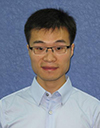
\includegraphics[width=1in,height=1.25in,clip,keepaspectratio]{Xueyong_Zhang.jpg}}]{Xueyong Zhang}
received the B.S. degree in applied physics from Nantong University, China, in 2011, the M.E. degree in microelectronics and solid-state electronics from Southeast University, China, in 2014, and the Ph.D. degree from Nanyang Technological University (NTU), Singapore, in 2022. From 2014-2016, he was a design engineer with Silergy Corp., where he was involved in power management IC design. From 2016-2022, he was a research associate and research fellow with NTU. He is currently a staff engineer with Huawei International Pte Ltd., Singapore. His current research interests include low-power analog IC, neuromorphic VLSI, in-memory computing design, and data converters.
\end{IEEEbiography}


\begin{IEEEbiography}[{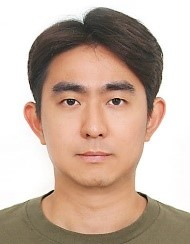
\includegraphics[width=1in,height=1.25in,clip,keepaspectratio]{ByungKwon.jpg}}]{Byung-Kwon An}
received the B.S. in Department of Electronics Engineering from Kwangwoon University, Korea, Seoul, South Korea, in 2017, He received the M.S degree in circuits for PCM Memories and OTS device from Hanyang University, Korea, Seoul, South Korea, in 2020. He is currently pursuing the Ph.D. degree in design circuits for RRAM Memories circuits with Nanyang Technological University, Singapore. His interests include design for circuit based on non-volatile memory.
\end{IEEEbiography}


\begin{IEEEbiography}[{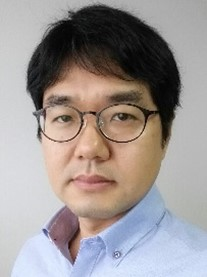
\includegraphics[width=1in,height=1.25in,clip,keepaspectratio]{ProfKim.jpg}}]{Tony Tae-Hyoung Kim}
(Senior Member, IEEE) received the B.S. and M.S. degrees in electrical engineering from Korea University, Seoul, Korea, in 1999 and 2001, respectively. He received the Ph.D. degree in electrical and computer engineering from the University of Minnesota, Minneapolis, MN, USA in 2009. From 2001 to 2005, he worked for Samsung Electronics where he performed research on the design of high-speed SRAM memories, clock generators, and IO interface circuits. In 2007 ~ 2009 summer, he was with IBM T. J. Watson Research Center and Broadcom Corporation where he performed research on isolated NBTI/PBTI measurement circuits and SRAM Mismatch measurement test structure, and battery-backed memory design, respectively. In November 2009, he joined Nanyang Technological University where he is currently an associate professor. His current research interests include in-memory computing for edge computing, emerging memory circuit design, energy-efficient circuits and systems for IoT and wearable devices, variation and aging tolerant circuits and systems, and circuit techniques for 3-D ICs .
He received Best Paper Award at 2021 ICCE-Asia, Best Demo Award at 2016 IEEE APCCAS, International Low Power Design Contest award at 2016 IEEE/ACM ISLPED, a best paper award at 2014 and 2011 ISOCC, 2008 AMD/CICC Student Scholarship Award, 2008 Departmental Research Fellowship from U. of Minnesota, 2008 IEEE DAC/ISSCC Student Design Contest Award, 2008 Samsung Humantec Thesis Award (Bronze Prize), 2005 ETRI Journal Paper of the Year Award, 2001 Samsung Humantec Thesis Award (Honor Prize), and 1999 Samsung Humantec Thesis Award (Silver Prize). He is an author/co-author of around 190 journal and conference papers and holds 17 US and Korean patents. He serves as an Associate Editor of IEEE Transactions on Very Large Scale Integration (VLSI) Systems, IEEE Access, Frontiers in Electronics, and IEIE Journal of Semiconductor Technology and Science (JSTS). He has also served as a technical committee member of various conferences such as IEEE Asian Solid-State Circuits Conference (A-SSCC), IEEE International Symposium on Circuits and Systems (ISCAS), IEEE/ACM International Symposium on Low Power Electronics and Design (ISLPED), etc. He is the Chair of IEEE CASS VSA-TC and was the Chair of IEEE SSCS Singapore Chapter in 2015~2016. He is an IEEE SSCS distinguished lecturer. He is a senior member of IEEE.
\end{IEEEbiography}



\end{document}